%%
%% This is file `thesis.tex',
%% generated with the docstrip utility.
%%
%% The original source files were:
%%
%% nudtpaper.dtx  (with options: `thesis')
%% 
%% This is a generated file.
%% 
%% Copyright (C) 2018 by TomHeaven <hanlin_tan@nudt.edu.cn>
%% 
%% This file may be distributed and/or modified under the
%% conditions of the LaTeX Project Public License, either version 1.3a
%% of this license or (at your option) any later version.
%% The latest version of this license is in:
%% 
%% http://www.latex-project.org/lppl.txt
%% 
%% and version 1.3a or later is part of all distributions of LaTeX
%% version 2004/10/01 or later.
%% 
%% To produce the documentation run the original source files ending with `.dtx'
%% through LaTeX.
%% 
%% Thanks LiuBenYuan <liubenyuan@gmail.com> for maintainence.
%% Thanks Xue Ruini <xueruini@gmail.com> for the thuthesis class!
%% Thanks sofoot for the original NUDT paper class!
%% 
%1. 规范硕士导言
% \documentclass[master,ttf]{nudtpaper}
%2. 规范博士导言
% \documentclass[doctor,twoside,ttf]{nudtpaper}
%3. 如果使用是Vista
% \documentclass[master,ttf,vista]{nudtpaper}
%4. 建议使用OTF字体获得较好的页面显示效果
%   OTF字体从网上获得,各个系统名称统一,不用加vista选项
%   如果你下载的是最新的(1201)OTF英文字体,建议修改nudtpaper.cls,使用
%   Times New Roman PS Std
% \documentclass[doctor,twoside,otf]{nudtpaper}
%   另外,新版的论文模板提供了方正字体选项FZ,效果也不错哦
% \documentclass[doctor,twoside,fz]{nudtpaper}
%5. 如果想生成盲评,传递anon即可,仍需修改个人成果部分
% \documentclass[master,otf,anon]{nudtpaper}
%
\documentclass[master,otf]{nudtpaper}

%%----DELETE-----%
%\usepackage{notes}
%\numberwithin{equation}{chapter}
%\numberwithin{figure}{chapter}
%%----DELETE-----%
%\usepackage{pdfpages}

\usepackage{lmodern}
\usepackage{mynudt}
\usepackage{multirow,array}

\classification{TP399}
\serialno{17060062}
\confidentiality{公开}
\UDC{004.8}
\title{基于自然语言处理的热点数据识别\\及应用技术研究}
%\title{基于自然语言模型的文件访问模式分析与文件预取方法研究}
\displaytitle{基于自然语言处理的热点数据识别及应用技术研究}
\author{陈辉}
\zhdate{\zhtoday}
\entitle{Research on Hot File Identification and Application Technology Based on Natural Language Processing}
\enauthor{Hui Chen}
\endate{\entoday}
\subject{计算机科学与技术}
\ensubject{Computer Science and Technology}
\researchfield{高性能计算}
\supervisor{周恩强\quad{}研究员}
\cosupervisor{}  % 协助指导教师,没有就空着
\ensupervisor{Prof. Enqiang Zhou}
\encosupervisor{} % 协助指导教师英文,没有就空着
\papertype{工学}
\enpapertype{Engineering}
% 加入makenomenclature命令可用nomencl制作符号列表。

\begin{document}
	\graphicspath{{fig/}}
	% 制作封面,生成目录,插入摘要,插入符号列表 \\
	% 默认符号列表使用denotation.tex,如果要使用nomencl \\
	% 需要注释掉denotation,并取消下面两个命令的注释。 \\
	% cleardoublepage% \\
	% printnomenclature% \\
\maketitle
\frontmatter
\tableofcontents
\listoftables
\listoffigures

\midmatter
\begin{cabstract}
分层存储是计算机存储领域的一项重要技术,其核心设计是将数据存储在多层级的存储介质中,通过热点文件识别和数据迁移技术来掩盖访问延迟以及增加吞吐率。分层存储管理的本质是准确、实时的文件分类,当存储层次较多时,可以转化为相邻层级之间热点数据和冷数据的二分类任务。文件分类的准确率十分依赖于对应用I/O行为的理解。本文工作主要包括以下两部分:

%1. 文件静态关联分析。我们提出了两条假设。第一条假设是POSIX文件系统的目录结构具有与自然语言相似的性质,即分布式语义假设。基于该假设,我们使用词嵌入模型将POSIX文件系统中的文件名、目录名映射为高维向量,以量化的方式分析它们之间的语义关联。第二条假设是一条完整路径的各级子向量可以线性相加,得到的结果可以近似表示该文件在文件系统空间中的位置。基于该假设我们提出了路径向量的概念。
文件关联分析。数据块关联性广泛存在于存储系统中,以往的研究通常从POSIX文件目录的树形结构入手,无法充分挖掘语义上的关联性。本文使用词嵌入模型将POSIX文件系统中的文件和目录映射为高维向量,将文件或目录之间的语义关联转化为向量空间中的内积计算,并通过降维可视化的方式予以直观呈现。
%2. I/O行为分析。在上述静态分析的基础上,我们提出了第三条假设:应用的I/O行为研究,可以转化为路径向量的序列分析问题。基于该假设,我们建立了循环神经网络来分析路径向量序列,最终用于解决文件的冷热分类任务,并利用GlusterFS中的tiring模块设计了一套智能分层存储管理的初步方案。

基于I/O行为分析的冷热文件分类。目前,该领域的研究通常局限于短期I/O请求序列的分析和预测,难以在较长时间跨度上挖掘应用的I/O行为模式。本文在文件和目录向量化表示的基础上,使用循环神经网络分析I/O请求序列,最终用于解决文件的冷热分类任务,并利GlusterFS文件系统中的tiring模块设计了一套智能分层存储管理的初步方案。

为验证模型的合理性,本文以开源工程代码编译为工作负载设计了文件冷热分类实验。实验结果表明,对于单进程编译任务,在经过参数调优后可以达到较高的热点文件识别率,且冷数据被误判的概率控制在较低水平。

\end{cabstract}
\ckeywords{分层存储;数据迁移;访问模式;词嵌入;循环神经网络}

\begin{eabstract}
Tierd storage is an import technology in the field of computer storage, which stores data in multiple tiers, masking latency and increasing throughput through file classification and data migration techniques. In fact, the main purpose of hierarchical storage management is to correctly classify files in runtime. When dealing with multi-tired storage system, this mission can be splitted into several sub-missions of binary classification. However, the correctness of file classification heavily depends on the understanding of the I/O behavior. Our research focuses on two aspects.

%Analysis on file correlations. In this part, we propose two assumptions. The first is the distributional hypothesis that the directory structure of POSIX file system is similar to natural language. Based on this hypothesis, we utilize word embedding model to map file names and directory names to high-dimension vectors, analyzing the semantic correlations among those names in a quantified manner. The other is that we could sum up those sub-vectors of a full path to approximately represent this path in the space of file system. Thus, we propose a concept named path vector. 

Analysis on file correlations. File correlations are common in storage systems. Recent researches in this area often focus on the tree structured directory of POSIX file systems which were unable to reveal the implicit semantic correlations among files and directories. We utilize word embedding model to map file names and directory names to high-dimension vectors, analyzing the semantic correlations among them by dot products. With the word embedding model trained, we show the semantic correlations with PCA and visualization.

%Sequential analysis on I/O behavior. Based on aforementioned works, we propose the third assumption, that the research on I/O behavior could be reframed to sequential analysis on path vectors. We build an RNN model to achieve this goal and design a hierarchical storage management solution based on tiering translator in GlusterFS.

File classification based on sequential analysis on I/O behavior. Recent works were not capable of long-term analysis. In this paper, based on aforementioned works, we build an RNN model to analyze the I/O behavior and design a hierarchical storage management solution based on tiering translator in GlusterFS.

To verify these models, we designed file calssification experiments with compiling workloads. The results show that our model performs well in single-process compiling, that the accuracy of hotspot indentification(recall rate) is good with fine-tuned hyperparameters, and the false positive rate controlled bellow.
\end{eabstract}
\ekeywords{Tiered Storage, Data Migration, Access Pattern, Word Embedding, RNN}



\mainmatter

\chapter{绪论}
\section{研究背景}
\textit{Stacker.}\linkout{stacker}{1}
\textit{Tiered Storage Systems}:\linkout{Adaptive_Data_Migration_in_Multi-tiered_Storage_Based_Cloud_Environment}{1}
\subsubsection*{分层存储技术}
分层存储系统(Tiered Storage System),又称为层级存储管理(Hierarchical Storage Management),是当前各领域存储系统的主流架构。其基本特点是将文件数据存储在若干层级的存储介质中,不同层级的介质(DRAM,SSD,HDD等)具有不同的容量、吞吐率、访问延迟与成本等。不同的应用负载和场景下,存储系统中的数据重要性存在差异,可以粗略地分为“热”数据与“冷”数据:正在访问与频繁访问的“热”数据优先存储于更接近CPU、访问更快的内存、SSD阵列等存储介质中;近期没有访问需求或访问频率低的“冷”数据主要存储在低层级的磁盘阵列或远程存储服务器中。在现实应用中,数据的“热”与“冷”不是静态的,而是随着应用的访问需求动态变化,数据在不同层级之间的迁移管理成为层次存储系统的基本任务之一。
\begin{figure}[htp]
    \centering
    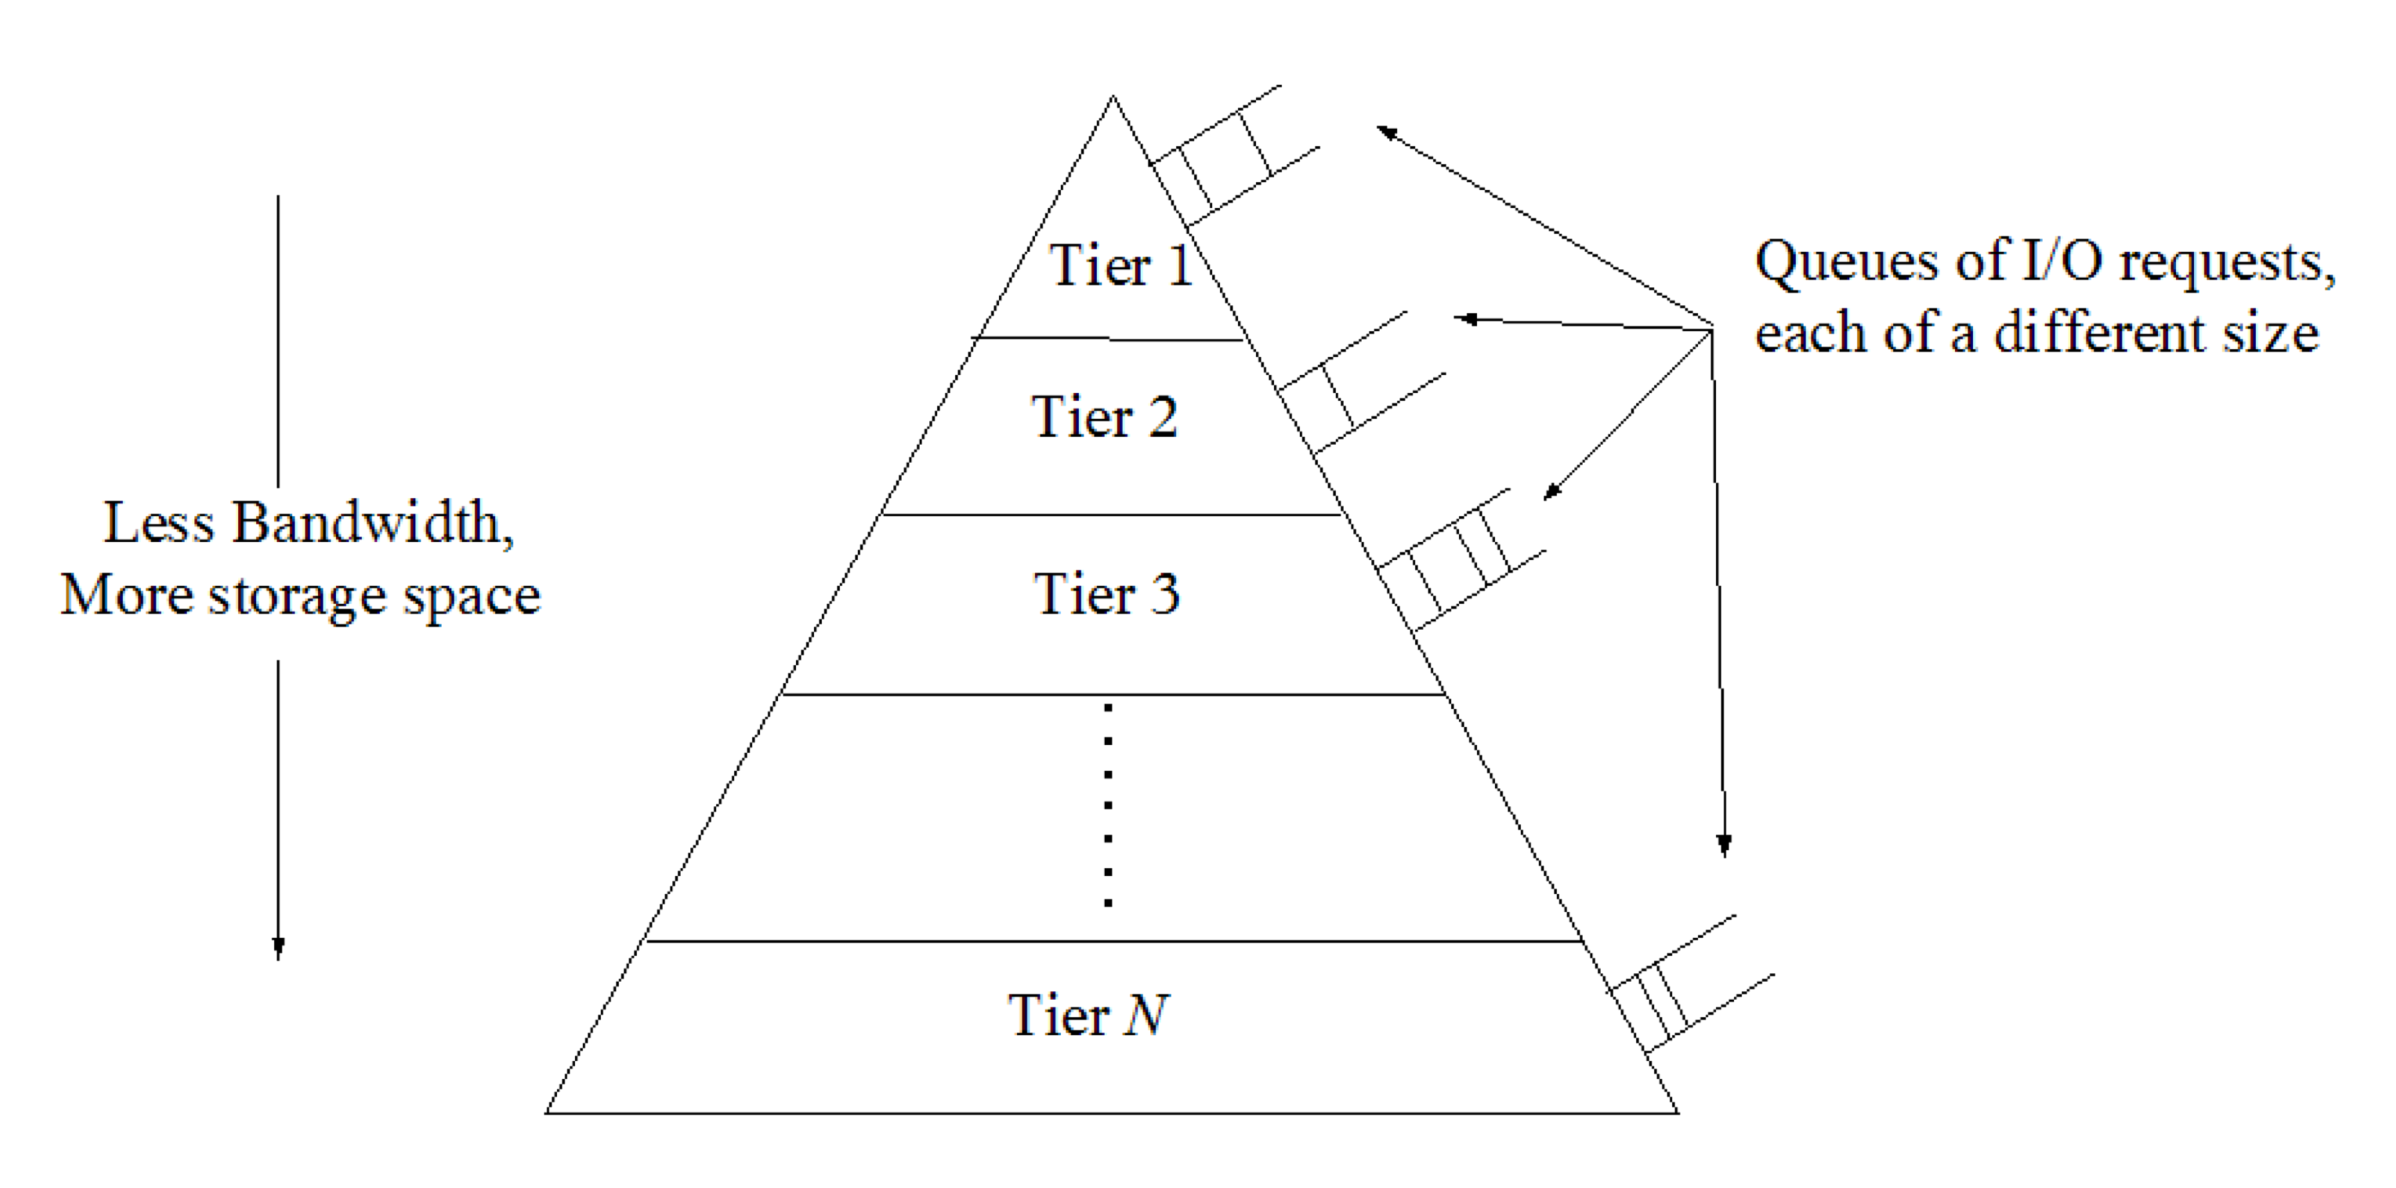
\includegraphics[width=\textwidth]{chp2_multi_tiers}
    \caption{分层存储系统(Tiered Storage System)}
    \label{fig:multi_tiers}
\end{figure}
如图\ref{fig:multi_tiers}所示,分层存储系统按层级从高到低由不同存储介质组成:
\begin{itemize}
    \item 高层级存储通常由内存DRAM(Dynamic Random Access Memory)、非易失性存储(Non-volatile Memory)等介质组成,其特点是读写性能优异、存储密度高,是实际应用场景中“热”数据的理想存储载体,同时也具有易失(DRAM)或寿命有限(NVM)等缺点
    \item 较低级存储通常由固态硬盘(Solid-State Driver)、磁盘(Hard Disk Drive)阵列组成,且在生产环境下这些存储阵列通常部署在远程存储服务器(Storage Servers),通过SANs(Storage Area Networks)或高速互联网络(InfiniBand)与客户端或计算服务器连接以提供存储服务。低层级存储性能较弱,存储密度较低,但同时也具有造价低廉、容量大、稳定性好的优点,且可以通过冗余磁盘阵列(Redundant Array of Inexpensive Disks)以及数据复制(Replication)等技术进一步提高数据的稳定性和容错能力。因此这类低层级存储是“冷”数据的理想载体。
\end{itemize}


近几十年来,分层存储在商业性数据存储领域得到了大规模应用。例如NetApp FAS系列存储系统
\cite{NetAppFas},
IBM DS8880
\cite{IBMDS8880}
等。这些支持Flash存储介质的存储系统方案主要可分为两类:第一类存储方案简单地将Flash存储介质作为较内存低一级的缓存
\cite{NetAppFas}
,以起到优化存储系统性能的作用。采用Flash存储介质作为缓存的主要优点是集成容易,不需要显式地考虑数据迁移策略,同时造价比DRAM低得多。第二类方案则是将Flash存储介质作为持续存储加入到层次存储结构中。

在大规模科学与工程计算领域,层次存储结构同样应用广泛。随着闪存技术的飞速发展,传统HPC所应用的三层技术架构(计算结点的共享内存-并行文件系统-归档存储)也随之发生变化。在HPC系统中,并行文件系统(pFS)对HPC性能影响非常大,在许多场景下决定了整个HPC的存储性能。传统HPC架构在应对超大规模HPC集群计算节点同时Checking Point需求时,显得力不从心,那就需要在pFS之上多加一层高速大容量(相对于Memory)的缓存(Burst Buffer)。典型代表有
{\color{red}此处补充采用Burst Buffer技术的超算架构}

\subsubsection*{分层存储架构中的数据迁移管理}
层次存储系统中的不同层级间的数据迁移管理是文件系统性能的关键。可粗略分为被动缓存和主动预取。预取(prefetching),也称为预分页(prepaging)或预读(read-ahead),是操作系统数据读取过程中的重要优化方法
\cite{Reducing_File_System_Latency_using_a_Predictive_Approach}
\cite{Group_based_management_of_distributed_file_caches}
\cite{A_data_mining_algorithm_for_generalized_web_prefetching}
。其目标是预测将来的数据访问,并在请求数据之前将其提前读取到高层级的存储介质中,从而起到掩盖访问延迟的作用。预取是传统缓存技术的一种补充,不同于被动数据迁移,预取技术的关键在于对即将访问的数据内容和生存周期进行主动预测。

\begin{itemize}
\item \textbf{“热”数据预测}:主动预取需要预测程序下一阶段可能访问的数据,是对数据访问的空间局部性的扩充。针对“热”数据准确的预测将极大地降低访问延迟,而错误预测将会引发浪费传输带宽,挤占缓存空间等负面影响。
\item \textbf{“热”数据生命周期预测}:与缓存机制中的时间局部性类似,主动预取需要针对缓存数据的时效性和生命周期建立有效的评估。非缓存数据的及时预取有助于提高存命中率,而清除短期内不再读取的数据将提高缓存空间的利用率。
\end{itemize}

预取的主要流程可总结如下:
\begin{enumerate}
\item 针对特定负载,提取访问日志;
\item 分析访问日志,对该负载的文件访问模式进行抽象表达;
\item 将负载的访问模式作为依据,引导文件系统进行主动预取。
\end{enumerate}

{\color{red}缓存vs预取概念对比图}

\section{国内外研究现状}
%\linkout{overview}{14}
Eshel等\cite{Panache}
提出并实现了缓存文件系统“Panache”,该系统使用pNFS以分布式缓存的方式存储GPFS中的缓存数据。
Frings等\cite{Massively_Parallel_Loading}
针对动态链接库加载过程进行数据预取,从而提高并行应用程序的性能。
Rajachandrasekar等\cite{1PB}
提出了一种用户级文件系统,将检查点请求保留在主内存中,并同时写入到持久性存储中。他们的方法包括对远程直接内存访问(RDMA)的支持。

Zhao等\cite{HyCache+}
提出了另一种缓存中间件,采用一种双阶段缓存技术来减少计算结点和I/O结点之间的数据传输量。
Isaila等\cite{Multi_Leve_Data_Staging_for_Blue_Gene}
提出了分别位于客户端和I/O节点之间,以及I/O节点和存储服务器之间的两级预取方案,从而改进了IBM Blue Gene的I/O转发层的数据传输性能。
Prabhakar等\cite{Adaptive_Multi_level_Cache_Allocation_in_Distribute_Storage_Architectures}
通过线性规划对两级缓存系统上的最佳缓存分配进行建模。

Kandemir等\cite{On_Urgency_of_I/O_Operations}
定义了I/O请求紧迫度的概念,该概念由请求可以延迟多长时间而不影响应用程序性能给出。在对I/O请求进行紧迫度分析后,通过优先处理紧急请求来改进缓存机制。
Seelam等\cite{Masking_IO_latency_using_application_level_IO_caching_and_prefetching_on_Blue_Gene_systems}
实现了能够追踪和分析应用I/O访问模式的库,并借此引导预取线程将数据提前读取到本地存储。
Patrick\cite{Cashing_in_on_Hints_for_Better_Prefetching_and_Caching_in_PVFS_and_MPI_IO},
He\cite{KNOWAC},
Tang\cite{Improving_read_performance_with_online_access_pattern_analysis_and_prefetching}
等提出了类似的方法(使用访问模式检测指导预取)。


Suei等\cite{Endurance_Aware_Flash_Cache_Management_for_Storage_Servers}
提出了一种使用SSD作为HDD缓存的存储集群缓存设计。其设计侧重于响应时间和缓存命中率。 

Welch和Noer\cite{Optimizing_a_hybrid_SSD_HDD_HPC_storage_system_based_on_file_size_distributions}
根据并行文件系统中小文件占多数的特点,将小文件存储在SSD中以优化对它们的访问。
He等\cite{Proceedings_of_the_22nd_international_symposium_on_High_performance_parallel_and_distributed_computing}
提出了一个代价模型来辅助数据迁移决策。该模型能够评估文件不同区域的访问成本,并将高成本区域放置在SSD中。

\section{本文主要工作}
\begin{itemize}
    \item 研究分析GlusterFS的原理、架构和功能实现,提出基于Tiering模块的数据迁移管理框架设计。
    \item 针对POSIX文件系统的目录结构、命名习惯等特点,提出采用词向量模型进行量化分析,即,将文件或目录映射到高维向量空间来分析文件、目录间的逻辑关系。
    \item 针对特定工作负载的I/O访问模式进行研究,在文件/目录向量化工作的基础上,采用循环神经网络提取和分析I/O访问模式,并用于替代传统的缓存算法(LRU等)指导GlusterFS进行数据迁移。
\end{itemize}
\section{论文结构}
% a)	不同存储层次存储介质,其性能和功能特点差异描述(数据、曲线),突出分层的意义。
% b)	缓存技术需要一个总结,阐明其问题缺陷,直接用于热点数据识别的劣势;
% 	主动预取,需要丰富若干文献;
% c)	本章篇幅少,广度和深度不够。



\chapter{相关工作介绍}
\section{分层存储}

所谓分层存储,是指由两种或更多种类型的存储组成的数据存储环境,其特点是各级存储之间的价格,性能,容量和功能这四个主要属性存在差异,从而在存储系统中扮演不同角色。近年来,随着存储容量的逐年提升和存储技术的迅速发展,这种层次化特点越来越鲜明:底端存储性能低,但具有超高容量和极低成本的优点;上层存储则具备非常高的性能水平和强大的数据管理功能,具备自动化数据管理功能的分层存储环境已成为一种必要的体系结构。分层存储系统的设计理念可以概括为:能够实现自动化的数据迁移,快速响应应用层的数据需求,以最低的代价获得最理想的综合性能。

%实际上,将效率与成本相同的存储介质部署在不同层级进行数据迁移复制在性能及成本上并不是有效的数据存储方式。因此,分层存储结构使用有差别的存储介质,以期在相同成本下,既满足性能的需要又满足容量的需要。这种存储介质上的差别主要是在存取速度上及容量上。存取速度快的介质通常都是存储单位成本(每单位存储容量成本,如1元/GB)高,而且容量相对来讲比较低。相应的,存取速度慢的介质通常是为了满足容量与成本方面的要求,既在相同的成本下可以得到更大的容量。所以,从这方面来说,分层存储其实是一种在高速小容量层级的介质层与低速大容量层级的介质层之间进行一种自动或者手动数据迁移、复制、管理等操作的一种存储技术及方案。

%此处应有举例说明{\color{orange}主要的存储供应商和许多新的存储厂商已经宣布计划或提供各种分层存储解决方案。 实际上,很少有供应商提供完整的分层存储产品组合,包括高性能SSD(固态磁盘),RAID阵列和归档磁带库。 实际上,许多供应商的分层产品都是“仅磁盘”策略,因为它们仅包括磁盘产品的RPM速度和价格范围的变化。 尽管这是大多数存储供应商都流行的分层存储方法,但是由于它迫使存档,活动量较小的数据驻留在不断旋转的磁盘上,因此无法有效地服务于第3层数据。 未使用的数据不应消耗能量。 请注意,企业不一定需要使用每个可用层,但是存储池越大,分层存储的好处就越大。}

\subsection{分层存储模型}
甲骨文公司关于分层存储研究报告\cite{Tiered_Storage_Takes_Center_Stage}指出,当前主流的分层存储模型可分为4个层级:

第0级:高性能存储。该层级是最接近计算结点的存储设备,存储的内容包括HPC应用,高性能数据库,数据库加速,索引、日志、卷文件、元数据存储等。该层级的存储介质通常为SSD(DRAM或闪存)。SSD提供极高的I/O性能,同时单位存储的造价也最高。

第1级:主要存储。主要存储层的存储内容为任务相关的关键数据,通常采用光纤通道技术(FC,Fibre Channel)将磁盘阵列连接组成区域存储网络(SAN,Storage Area Network)。该层级存储提供高性能、低延迟、高可用性和快速数据恢复等特性,可以快速稳定地为各类任务提供存储服务。

第2级:次级存储。次级存储的主要任务是存储相对重要的数据,例如常规的数据库、数据备份等等。该层次的数据I/O性能要求相对较低,注重易用性、易管理性、可扩展性和相对较低的成本,因此通常采用以太网连接磁盘阵列组成附加存储网络(NAS,Network Attached Storage)。

第3级:长期存储。该层级是存储系统中的最底层,存储对象是长期存档数据,例如社交网络存档数据、安保视频数据以及大规模科学计算中的归档数据等。此类数据总容量极大,访问频率低,具有一次写入多次读取(Write-Once-Read-Many)的特点,几乎没有I/O性能要求,因此磁带存储(Tape Storage)和近年兴起的蓝光光盘是最理想的存储介质。

\begin{table}[htbp]
\centering
\begin{minipage}[t]{0.9\linewidth}
\caption{典型分层存储模型}
\label{tab:TS_model}
\begin{tabularx}{\linewidth}{cZcZcZcZ}
\toprule[1.5pt]
{\hei 存储层级} & {\hei 第0级} & {\hei 第1级} & {\hei 第2级} & {\hei 第3级} \\
\midrule[1pt]
容量占比 & 1-3\% & 12-20\% & 20-25\% & 43-60\% \\
\hline
主要存储技术 & SSD & FC-SAN & NAS & 磁带库,蓝光存储 \\
\hline
数据类型 & I/O密集型 & 任务关联型 & 重要、敏感 & 长期归档 \\
\hline
I/O性能要求(IOPs) & >$10^6$ & 200-300 & 100-200 & 极低 \\
\hline
容灾指标RPO(小时) & <4 & <4 & <12 & 一天以上 \\
\hline
容灾指标RTO(小时) & <1-2 & <1-2 & <5 & <24 \\
\hline
功耗 & 低 & 最高 & 高 & 最低 \\
\bottomrule[1.5pt]
\end{tabularx}
\end{minipage}
\end{table}

\subsection{数据分类}
对于数据管理者来说,应当应用实际需求对文件数据分类,以匹配存储层级的方式对数据进行管理。与0-3层存储层级相对应,数据可分为以下4类:

I/O密集型数据。此类数据在所有文件中容量占比大约为3\%,主要包括对响应时间要求严苛的应用与文件,由于对I/O性能的优先级最高,因此存放在第0层。例如高性能操作系统文件、HPC应用、高性能数据库以及索引、日志、目录文件等元数据文件。

任务关联型数据。此类数据是指与正在运行的应用直接关联的数据,容量占比大约12-20\%,存放在第0级或第1级以保证应用的正常运行。这类数据对容灾能力要求较高,数据恢复时间(Recovery Time Objective,RTO)通常在几分钟到1-2小时。另一方面,当切换至不同的应用负载时,应及时将相关数据从第2级迁入到第0-1级。任务关联型数据包括任务相关的数据库、虚拟机、在线交易系统等等。


重要与敏感数据。这类数据不会直接影响应用的正常运行,因此通常存储于第2级,容量占比大约20-25\%。容灾能力要求较宽松,通常恢复时间允许在4小时以内。这类数据包括数据库、网络服务和应用、数据备份、恢复与数据安全系统、云存储等。

归档数据。归档数据容量占比最高,约占总容量的43-60\%,也是容量增长速度最快的一类数据。归档数据的访问频率最低,部分具有一次写入多次读取的特点,对I/O性能和容灾要求最低,通常存储在最底层的第3层。例如长期备份数据、离线媒体类数据、非结构化的文档数据以及大规模科学工程计算归档数据等。

\subsection{分层存储管理}
分层存储管理(Hierarchical Storage Management,HSM)是指对存储系统中所有数据统一管理调度,根据数据的访问频率、性能要求等因素进行实时分类,并在不同层级之间自动迁移的技术。在上述分层存储模型与数据分类方式下,分层存储管理方案的优劣直接决定了存储系统的整体性能与性价比。

在实际的分层存储管理方案设计中,4分类问题可化为多次二分类任务,即,任意相邻的两个层级分别视为热存储和冷存储,数据的迁移策略由冷热分类的结果决定。分类指标可总结如下:

I/O性能要求。这里的性能要求特指访问延迟,或者说每秒访问次数(IOPs),例如文件元数据,数据库索引文件等访问延迟越低越好。

任务关联性。任务关联性是指,特定的应用在生命周期中的某一阶段,部分数据是该应用即将访问或频繁访问的,这些数据属于任务关联型数据;而其他数据在较长时间内不会被访问,任务关联性较低。

各级存储容量比例、功耗要求、容灾能力。这些指标属于硬件条件等外部环境,决定了数据分类的具体阈值。例如,高性能存储介质的容量高,意味着更多的元数据文件或任务关联型数据可以存放在第0级或第1级;功耗要求严格,意味着需要避免错误分类,减少数据迁移;容灾恢复时间(RTO)短,意味着这部分数据需要在较高层级的存储介质中进行备份。

在本课题中,我们主要针对任务关联性指标展开研究,主要研究对象是第0-1层与第2层之间的数据二分类与迁移策略。在实际应用背景下,数据的任务关联性是随着程序运行动态变化的,良好的分层管理方案应能侦测应用的长期访问模式,并准确识别热点数据指导数据迁移。为此,在后续研究中,我们针对POSIX文件系统建立了路径嵌入模型,以量化分析文件之间的静态关联;在此基础上,建立循环神经网络分析特定应用负载的I/O行为,挖掘数据与应用运行时的动态关联规律,并以此为依据进行文件的冷热分类实验。


\section{自然语言处理相关技术}
自然语言处理(NLP)的定义可以简单概括对人类语言进行自动化、智能化分析以及学会人类表达的一系列计算机技术,是一门包含着计算机科学、时间序列分析以及语言学的交叉学科,这些学科既有区别又相互交叉。

1936年A.M.Turing发明了举世闻名的“图灵机”,使数学中的逻辑符号和真实世界之间建立了联系,为后来计算机的蓬勃发展提供了坚实的理论基础。20世纪50年代,在图灵机的计算模型的基础上,自动机理论被提出,是现代计算机科学发展的基础\cite{自然语言处理的历史与现状}。后来Kleene又在自动机理论模型之基础上提出了正则表达式和有限自动机。1956年,Chomsky提出了上下文无关的语法的理论,同年人工智能被发明后,被迅速应用到自然语言处理领域之中。上下文无关语法的提出使得该领域的研究分为了基于推理规则的符号派和基于概率论的随机派\cite{宋一凡2019自然语言处理的发展历史与现状},在之后很多年里分别高速发展。70年代语音识别算法研制成功,隐马尔科夫模型(Hidden Markov Model,HMM)提出并得到了广泛应用\cite{自然语言处理的历史与现状}。

近年来,随着深度学习的飞速发展,自然语言处理领域也取得了诸多重要突破。RonanCollobert等\cite{Natural_language_processing_(almost)_from_scratch}于2011年的研究提出了一个简单的深度学习框架,在许多NLP经典任务中取得了前所未有的性能,如实体命名识别、语义标注和词性标注等。之后,研究人员提出了大量基于复杂深度学习的算法,用于解决有难度的NLP任务。2013年,Mikolv\cite{skipgram}提出了当前NLP领域最重要的模型之一Skip-gram,该模型以出色的性能表现将单词转化为高维向量,为后续如雨后春笋般涌现的自然语言处理模型奠定了基础。

本章后续内容以词嵌入方法、循环神经网络等主流自然语言处理模型为基础,探讨其在文件系统优化,尤其是数据迁移策略中“冷”、“热”文件分类问题的应用。

\subsection{词嵌入}

%\href{https://www.linkresearcher.com/careers/6c7a15b5-236a-40f3-879f-af2ac06c2557}{NLP综述博客}
%\href{https://blog.csdn.net/mawenqi0729/article/details/80698350}{词嵌入博客}

众所周知,在自然语言处理任务中,第一步工作就是用计算机能够理解的方式表示和描述单词,也就是将其用向量表示。通常有两大类表征方式:离散型表示(one-hot)和分布型表示(distributed representation)。

所谓离散型表示是指,在给定词汇表$V$的条件下,每一个单词被表示为一个维度为$|V|$的向量,该词汇表中任意一个单词,唯一地分配一个维度为1,其余维度均为0。例如单词file在词汇表中第二个出现,则其离散型向量表示为:$v_{file} = [0,1,0,\dots,0]$。这种表示方式相当于为每个单词分配了一个唯一的ID。当词汇表较大时,词嵌入的维度将会非常高,并且无法表达词与词之间的关系。

单词的分布式表示基于语义学中的分布式假设(Distributional Hypothesis)\cite{distributional_hypothesis}:
在相似的上下文中出现的单词通常具有相似的含义。例如单词water和coffee常与drink搭配,因此water与coffee具备一定的的相似性。分布式表示的目的就是将单词转化为稠密的向量(与离散型的one-hot向量相对),将人类自然语言中的单词之间的相似性和逻辑关联转化为向量空间的数学关系来处理(例如使用二范数表达单词的相似度)。见图\ref{fig:t_sne}所示例子,Li等人\cite{visualizing}采用t-SNE方法对60维的词嵌入进行降维处理,结果显示,含义相近的单词在向量空间内“距离”也比较接近。
\begin{figure}[htp]
\centering
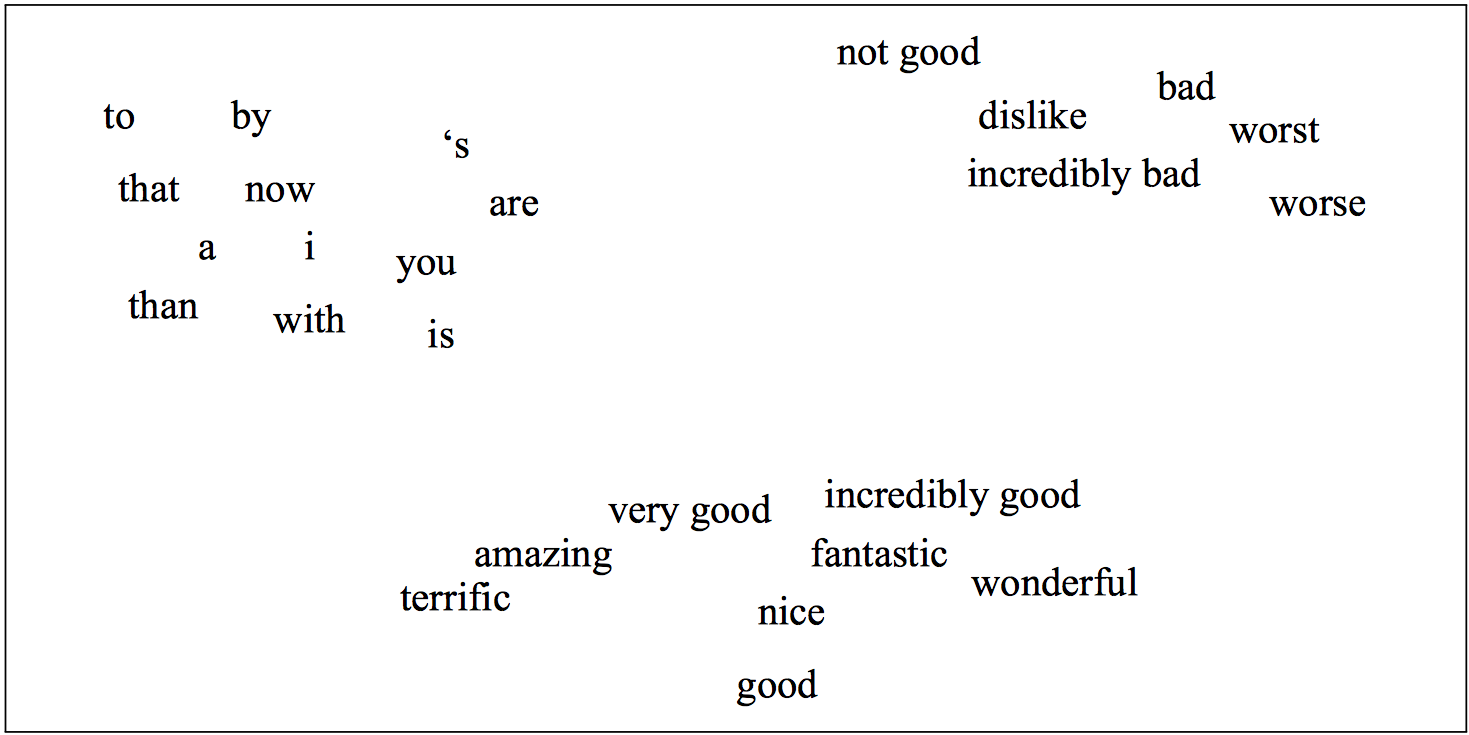
\includegraphics[width=\textwidth]{t_sne}
\caption{词向量降维后的可视化}
\label{fig:t_sne}
\end{figure}
%{\color{red}词嵌入降维图}\linkout{nlp_book}{107}

%{\color{red}词嵌入相关文献}\linkout{nlp_book}{128}

为实现这种从自然语言到向量空间的映射,自然语言处理发展历史上出现了许多理论和方法,例如Deerwester于1988年提出的潜在语义索引(Latent Semantic Indexing)方法\cite{LSI},以及该作者后续应用奇异值分解(SVD)对共现矩阵降维而实现的潜在语义分析方法(latent semantic analysis)\cite{LSA},在此后多年里被广泛应用于多种NLP任务,如认知模型\cite{cognitive_model},拼写检查\cite{spell_checking},写作评分\cite{essay_grading}等等。

随着近年来深度学习的发展,基于神经网络的自然语言模型开始流行,Bengio分别在2003年\cite{bengio2003}和2006年\cite{bengio2006}发表的成果表明,神经网络语言模型能在单词预测任务中出色地担任词嵌入转换的角色。

2013年,Mikolov提出了著名的连续词袋(CBOW)和Skip-gram模型\cite{skipgram},可以说这两种词嵌入模型的发明引发了NLP领域的深刻变革,至今为止这两种模型组成的Word2Vec方法仍被广泛使用于学术界和工业界。

Word2Vec是以无监督的方式从海量文本语料库中学习语义知识的一种模型,已被广泛应用在自然语言处理中。那么其实现的原理是怎样的?Word2Vec的根本原理是用词向量的方式表征词与词之间的语义信息,即通过将单词映射到一个高维空间来表征相近词之间的关联。这里的映射就是词嵌入。

Word2vec中实现的词向量训练方式有两种,Skip Gram和CBOW(constinuous bags of words),其中Skip Gram根据目标单词对上下文可能出现的单词进行预测,CBOW则相反,它通过上下文预测目标单词,最后使用模型的部分参数作为词向量。接下来,本文以Skip-gram算法为例进行原理介绍。

假设语料库中单词总数为$T$,其词汇表$\mathcal{V}$中的词汇数量为$W$。
%其中任意一个词可用其在词汇表中的序号表示:$w \in \{1,\dots,W\}$。
那么该语料库可表示为一个由$T$个词向量组成的序列:$\mathbf{w}_1, \mathbf{w}_2, \dots, \mathbf{w}_T$。Skip-gram模型的目标就是建立一个从该词汇表中所有文件名和目录名到$d$维向量空间的映射$model:\mathcal{V} \rightarrow \mathbb{R}^d$,使以下对数极大似然函数达到最大:
\begin{equation}
    \label{eq:origin_object}
    \frac{1}{T}\sum_{t=1}^T \sum_{c \in \mathcal{C}_t} \log p(\mathbf{w}_c | \mathbf{w}_t),
\end{equation}
取负号得到损失函数:
\begin{equation}
    L(\theta)= -\frac{1}{T}\sum_{t=1}^T \sum_{c \in \mathcal{C}_t} \log p(\mathbf{w}_c | \mathbf{w}_t),
\end{equation}

其中,$\mathcal{C}_t$表示某中心词$\mathbf{w}_t$的上下文中出现过的词的集合。对于任意样本$(\mathbf{\mathbf{w}}_t,\mathbf{\mathbf{w}}_c)$,我们可用归一化函数softmax来定义单词$\mathbf{w}_c$在中心词$\mathbf{\mathbf{w}}_t$的上下文中出现的条件概率:
\begin{equation}
    \label{eq:softmax}
    p(\mathbf{w}_c | \mathbf{w}_t)=\frac{ e^{ \mathbf{w}_t^{\top} \mathbf{w}_c} }{ \sum_{j=1}^W e^{\mathbf{w}_t^{\top} \mathbf{w}_j}} 
\end{equation}

Skip-gram模型是一个三层神经网络,输入为词汇表中单词的初始向量,即$W$维的one-hot编码。隐层由$d$个神经元组成,没有激活函数,只有权值。训练收敛后隐层的$W\times d$的权值矩阵就是词汇表内所有词向量的集合。输出层为上文所述的softmax函数,最终结果是一个$W$维的向量,每个分量表示对应的单词与输入词存在上下文关系的概率。

当语料库规模较大,词汇表内单词较多时,采用softmax函数的计算复杂度过高。一种优化方式是使用层次化softmax(Hierarchical softmax)\cite{Hierarchical_softmax}。另一种计算复杂度更低,且同样能保证对原有softmax层拟合精度的优化方式是负采样(Negative sampling)。该方法将原来的预测上下文的问题转化为一系列独立的二分类问题,即,在选定中心词后,对词汇表中其他单词依次判定是否在中心词附近出现。


对任意中心词$\mathbf{w}_t$,用交叉熵损失函数(Cross-entropy Loss)代替原来的损失函数
\begin{equation}
    \label{eq:loss_of_t}
    L_t(\theta) = -\left( 
        \sum_{c \in \mathcal{C}_t} \log(p(\mathbf{w}_c | \mathbf{w}_t))+\sum_{c \in \mathcal{N}_t} \log(1-p(\mathbf{w}_c | \mathbf{w}_t)) 
    \right)
\end{equation}
其中$\mathcal{C}_t$表示中心词$w_t$的上下文单词集合(正样本),$\mathcal{N}_t$表示词汇表中,与$w_t$不存在上下文关系的单词(负样本)中随机抽取的若干噪声词。

由于任意单词与中心词是否上下文被视为独立事件,可用sigmoid函数拟合条件概率
\begin{equation}
    p(\mathbf{w}_c | \mathbf{w}_t) = \frac{1}{1+e^{-\mathbf{w}_t^{\top} \mathbf{w}_c}} = \sigma(\mathbf{w}_t^{\top} \mathbf{w}_c)
\end{equation}

代入\ref{eq:loss_of_t}并按$t$累加求平均,得到最终的损失函数:
\begin{equation}
    L(\theta) = -\frac{1}{T}\sum_{t=1}^{T} \left[
        \sum_{c \in \mathcal{C}_t} \log(\sigma(\mathbf{w}_t^{\top} \mathbf{w}_c)) + \sum_{c \in \mathcal{N}_t} \log(\sigma(-\mathbf{w}_t^{\top} \mathbf{w}_c))
    \right]
\end{equation}

在Word2Vec中,无论是连续词袋模型还是Skip-gram,都将单词作为基本单元,为每一个单词生成一个向量。这种映射方式使得单词内部的形态和构造特征被忽略。与此同时,Word2Vec对陌生或低频单词的嵌入支持不好,当遇到语料库之外的单词时效果不好。

FastText的出现弥补了Word2Vec这些缺点。该模型采用字符级别的n-gram来表示单词,即,每个单词都是由子词(subword)构成,这些子词被以n-gram的形式存储和使用。基于字词建模后,完整单词的向量由其包含的字词向量相加得来。


\subsection{循环神经网络概述}
%简述RNN发展情况

循环神经网络最核心的功能是处理和预测序列类型的数据。在全连接神经网络或卷积神经网络模型中,网络的结构通常由输入层、隐藏层以及输出层构成,输入的样本数据相互独立,没有前后联系。而循环神经网络的功能结构有着本质区别,隐藏层之间的节点是有连接的,隐藏层的输入不仅仅由输入层的输出决定,还包括前一时刻隐藏层输出的隐状态,临近的样本数据包含的数据得以保持,因此具备了处理序列数据的能力。

\begin{figure}[htp]
\centering
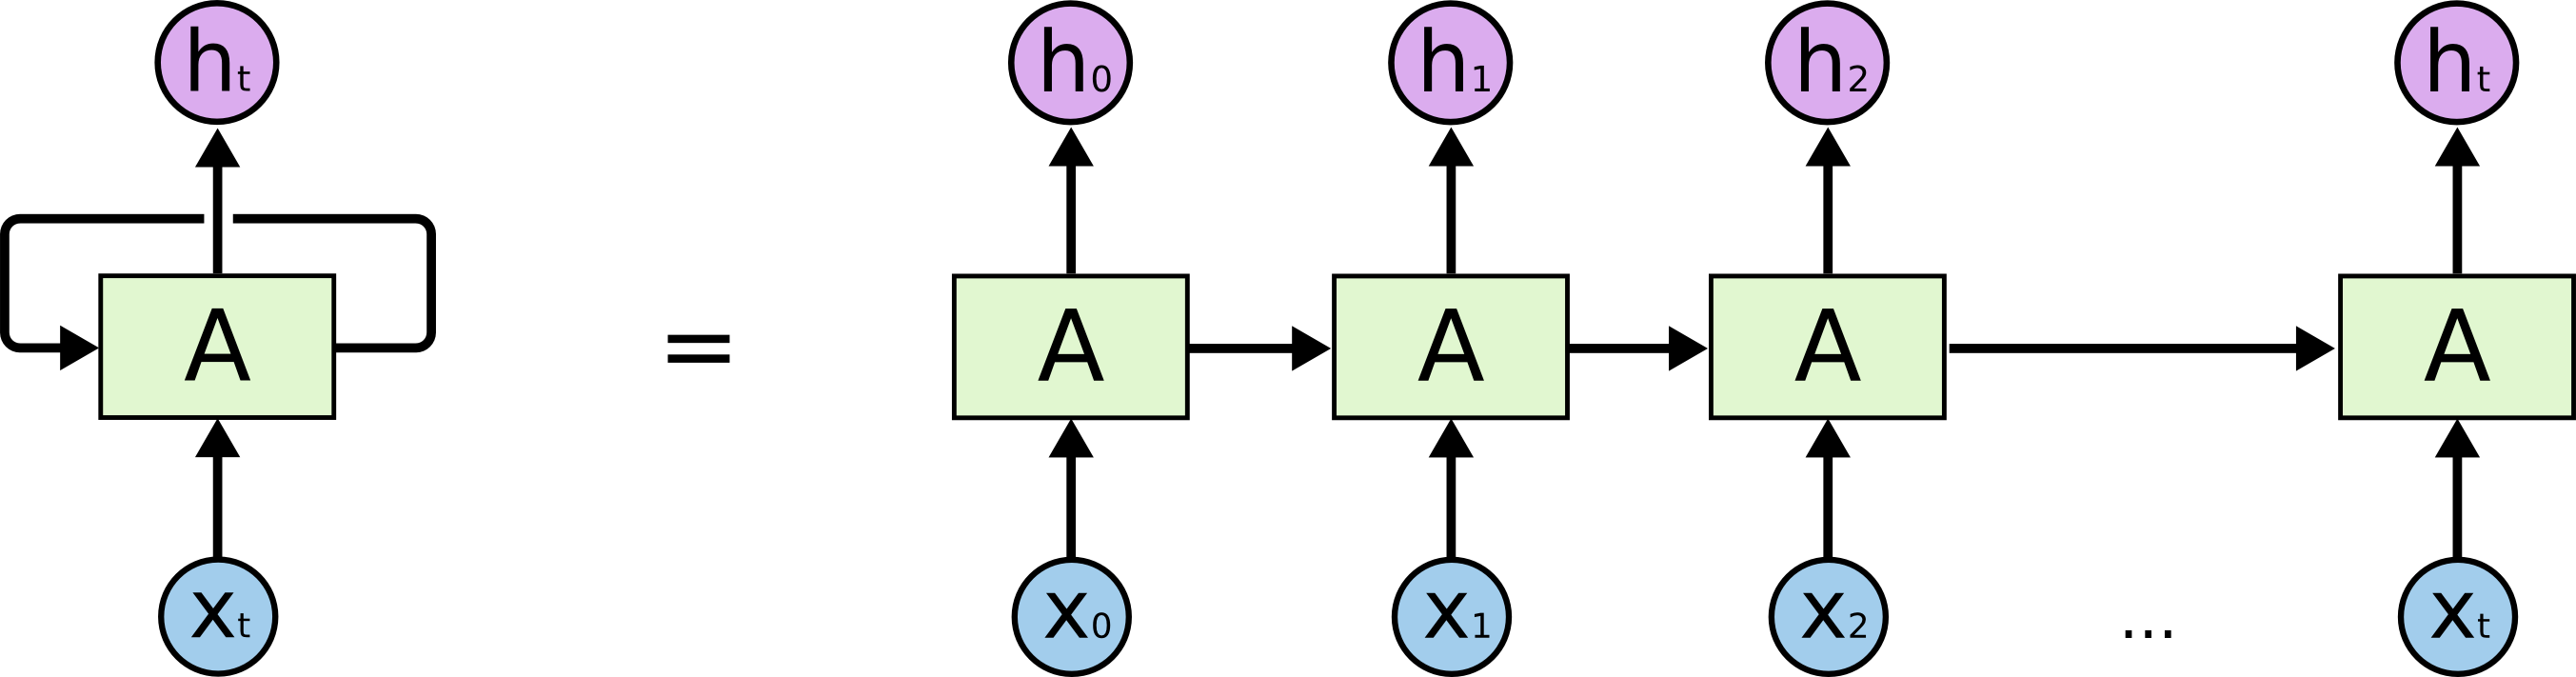
\includegraphics[width=\textwidth]{rnn_1}
\caption{RNN展开后的结构}
\label{fig:rnn_1}
\end{figure}
循环神经网络中区别于全连接或卷积神经网络的一个重要的概念就是时刻,输入数据以时间为标记。循环神经网络展开后如图\ref{fig:rnn_1}显示,除了来自输入层的样本数据$X_t$,还有一部分由前一时刻隐状态的计算结果提供。在每一个时刻,循环神经网络的运算单元会读取t时刻的输入$X_t$,并输出一个隐状态值$H_t$,同时将该隐状态传递到下一步。循环神经网络理论上可看作是一系列数据通过同一网络结构循环计算的结果。RNN根据输入输出对应关系可分为如下几类:

\begin{figure}[htp]
\centering
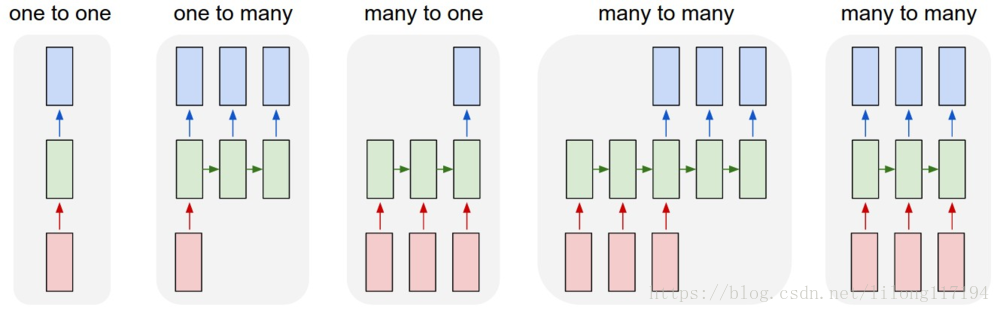
\includegraphics[width=\textwidth]{rnn_2}
\caption{RNN的多种模式}
\label{fig:rnn_2}
\end{figure}
%与常规的神经网络相比,循环神经网络以序列数据为输入,输出对应的序列数据结果。如图\ref{fig:rnn_2}所示,每一个矩形是一个向量,箭头则表示函数(如矩阵相乘)。输入向量用红色标出,输出向量用蓝色标出,绿色的矩形是RNN的状态。

1)单一输入和单一输出的Vanilla模型,例如图像分类任务;

2)单一输入序列输出,例如通过图片生成字幕;

3)序列输入单一输出,如自然语言情感分类任务,给定语句判断为积极或消极标签;

4)序列输入和序列输出,例如机器翻译任务;

5)同步输入输出,如视频分类任务。



%。其前向传播计算公式如下:
%\begin{align*}
%    r_t &= \sigma(W_r \cdot [h_{t-1},x_t]) \\
%    z_t &= \sigma(W_z \cdot [h_{t-1},x_t]) \\
%    \tilde{h_t} &= \tanh(W_{\tilde{h_t}}) \cdot [r_t \odot h_{t-1},x_t]) \\
%    h_t &= (1-z_t) \odot h_{t-1} +z_t \odot \tilde{h_t} \\
%    y_t &= \sigma(W_o \cdot h_t)
%\end{align*}
%其中方括号表示两个向量连接,$\odot$表示矩阵逐点相乘。
%

\subsection{本章小结}
本章第一节明确了分层存储的定义,并对当前主流的4层存储模型进行了阐述。与4层存储模型相对应的是数据的分类方式,主要包括I/O密集型、任务关联型、重要与敏感数据、归档数据等。在此存储模型下,数据分类的指标可归结为I/O性能要求、任务关联性以及外部环境要求等三方面。我们的研究针对任务关联性指标展开,为了捕捉文件之间的静态关联和较长时间跨度的任务关联性,本文建立了词嵌入模型和基于循环神经网络的模型,将在后续章节中逐一介绍。

第二节对自然语言处理领域的两个重要内容进行了介绍,一是词嵌入技术的发展概况和基本原理,尤其是近年来广泛应用的Word2Vec模型。二是介绍了循环神经网络的基本概况,阐明其在自然语言处理和序列处理中的广泛应用。随后阐述了LSTM神经网络基本原理及其解决长期依赖问题的特性。
%分层存储和自然语言处理合并为一章:相关工作介绍,质量可以适当降低。
% 引言:概述分层存储特点-》分层存储管理的重要性->j
% 2.1 分层存储
% 	2.1.1 分层存储模型
% 	2.1.2 数据分类
% 	2.1.3 分层存储管理
% 		数据关联挖掘;N-GRAM模型;缺陷
% 2.2 自然语言处理相关技术
% 	2.2.1 词嵌入:突出词嵌入能表达语义关联的特性;可视化展现;
% 	2.2.2 循环神经网络:突出RNN在序列分析中的作用。举例LSTM用于内存访问预测的论文;

\chapter{理论模型}
\section{利用词嵌入技术构造新型元数据}
\subsection{文件名、目录名的向量化}
在Unix文件系统中,任意文件或目录在被创建时,均会被分配一个唯一的ID,也就是Inode序号,以此作为唯一的标识以便于后续各种文件操作。Inode序号只与文件创建先后相关,是一种one-hot的表示方式。那么能否效仿自然语言处理中词嵌入的思想,建立一种能够包含文件或目录之间关联性的表征方式?

文件系统层次结构规范(Filesystem Hierarchy Standard,FHS)\cite{fhs}是由Linux基金会在1994年发起,旨在规范Linux各发行版和其他类Unix系统下文件目录结构的业界统一标准,至今已发展演变到FHS-3.0(2015年)。在FHS定义的目录结构规范下,Linux操作系统的目录组织结构和命名受到了明确严格的约束,例如:

{\color{red}这里做成表格!}
\begin{itemize}
    \item /:根目录。
    \item /bin:系统执行文件目录。
    \item /boot:启动文件目录。
    \item /dev:驱动设备目录。
    \item /etc:系统配置文件目录。
    \item /lib, /usr/lib, /usr/local/lib:系统使用的函数库目录。
    \item ......
\end{itemize}

如果将一个文件的完整路径(如/usr/lib/python2.7/)视为一个句子,各级目录视为单词,我们假定类似于自然语言中的分布式假设同样成立,即:同一目录下的文件或目录具有类似的含义。直观上看,这个假设是合理的,例如/bin目录下的bash,rm,cp文件等均为可执行命令,/usr/lib/python2.7/目录下均为Python的库文件。在此假设成立的前提下,本节将介绍如何使用Skip-gram模型,对给定的Unix文件系统目录下所有文件名、目录名进行向量化。

\subsubsection*{语料库的生成}
众所周知,任何机器学习模型都离不开数据,自然语言处理领域的数据集通常被称为语料库(Corpus)。任何语言学的研究或者自然语言模型的建立都必须建立在大量的语料之上,否则无论是基于规则方法还是统计方法建立的模型都将失效。

为了建立文件路径相关的“语料库”,我们将从根目录(或文件系统的挂载点)开始,通过常规的遍历算法将此目录下所有文件、目录的完整路径逐行写入到一个文本文件,作为模型的训练数据集。语料库生成后,相应地可以得到一个词汇表$V$。
{\color{red}此处插入遍历算法}

\subsubsection*{利用Skip-gram模型训练文件和目录名的词向量}
给定总单词数量为$T$的语料库,其词汇表$\mathcal{V}$=\{\textit{bin,boot,dev,...}\},词汇数量为$W$。
%其中任意一个词可用其在词汇表中的序号表示:$w \in \{1,\dots,W\}$。
那么该语料库可表示为一个由$T$个词向量组成的序列:$\mathbf{w}_1, \mathbf{w}_2, \dots, \mathbf{w}_T$。Skip-gram模型的目标就是建立一个从词汇表到$d$维向量空间的映射$model:\mathcal{V} \rightarrow \mathbb{R}^d$,使以下对数极大似然函数达到最大:
\begin{equation}
    \label{eq:origin_object}
    \frac{1}{T}\sum_{t=1}^T \sum_{c \in \mathcal{C}_t} \log p(\mathbf{w}_c | \mathbf{w}_t),
\end{equation}
取负号得到损失函数:
\begin{equation}
    L(\theta)= -\frac{1}{T}\sum_{t=1}^T \sum_{c \in \mathcal{C}_t} \log p(\mathbf{w}_c | \mathbf{w}_t),
\end{equation}

其中,$\mathcal{C_t}$表示某中心词$\mathcal{w}_t$的上下文中出现过的词的集合。以路径\textit{/usr/local/lib/python}为例,若取上下文窗口大小为1,那么中心词$\mathcal{w}_t$=\textit{lib}的上下文集合$\mathcal{C_t}$=\{\textit{local,python}\},在文件系统的情境下,此处“上下文”隐含的语义是指\textit{usr},\textit{python}分别与\textit{lib}有着父子目录的关系。对于任意样本$(\mathbf{\mathcal{w}}_t,\mathbf{\mathcal{w}}_c)$,我们可用归一化函数softmax来定义单词$\mathcal{w}_c$在中心词$\mathbf{\mathcal{w}}_t$的上下文中出现的条件概率:
\begin{equation}
    \label{eq:softmax}
    p(\mathbf{w}_c | \mathbf{w}_t)=\frac{ e^{ \mathbf{w}_t^{\top} \mathbf{w}_c} }{ \sum_{j=1}^W e^{\mathbf{w}_t^{\top} \mathbf{w}_j}} 
\end{equation}

\begin{figure}[htp]
\centering
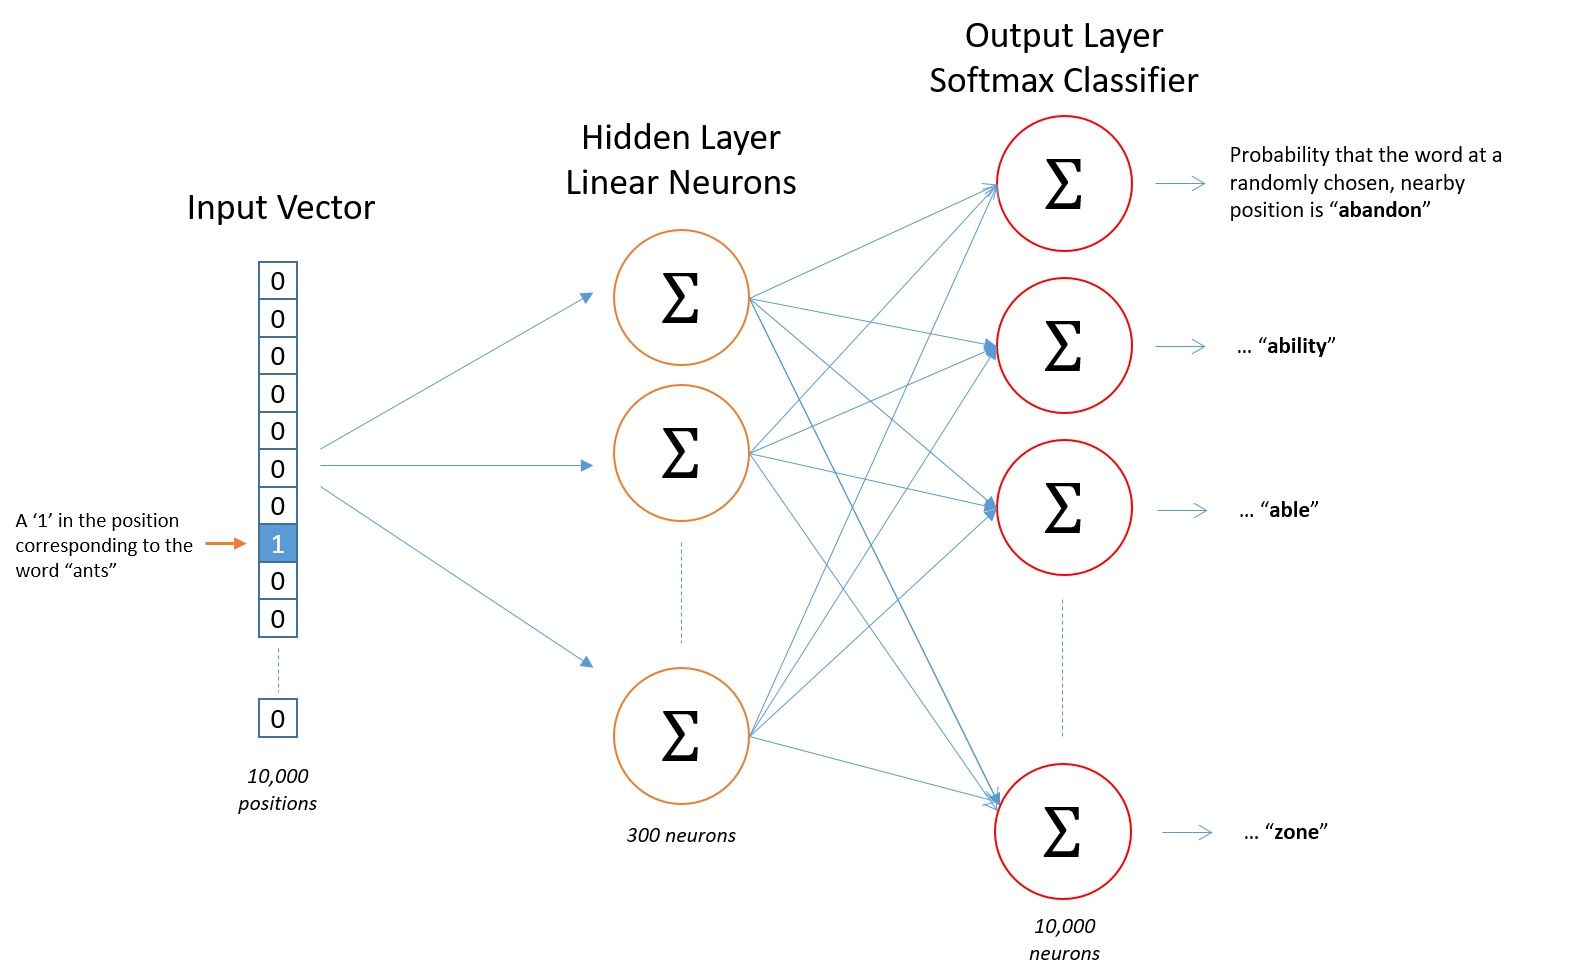
\includegraphics[width=\textwidth]{word2vec_nn}
\caption{Skip-gram模型网络}
\label{fig:word2vec_nn}
\end{figure}
如图\ref{fig:word2vec_nn},Skip-gram模型是一个三层神经网络,输入为词汇表中单词的初始向量,即$W$维的one-hot编码。隐层由$d$个神经元组成,没有激活函数,只有权值。训练收敛后隐层的$W\times d$的权值矩阵就是词汇表内所有词向量的集合。输出层为上文所述的softmax函数,最终结果是一个$W$维的向量,每个分量表示对应的单词与输入词存在上下文关系的概率。

当语料库规模较大,词汇表内单词较多时,采用softmax函数的计算复杂度过高。一种优化方式是使用层次化softmax(Hierarchical softmax)\cite{Hierarchical_softmax}。另一种计算复杂度更低,且同样能保证对原有softmax层拟合精度的优化方式是负采样(Negative sampling)。该方法将原来的预测上下文的问题转化为一系列独立的二分类问题,即,在选定中心词后,对词汇表中其他单词依次判定是否在中心词附近出现。


对任意中心词$\mathbf{w}_t$,用交叉熵损失函数(Cross-entropy Loss)代替原来的损失函数
\begin{equation}
    \label{eq:loss_of_t}
    L_t(\theta) = -\left( 
        \sum_{c \in \mathcal{C}_t} \log(p(\mathbf{w}_c | \mathbf{w}_t))+\sum_{c \in \mathcal{N}_t} \log(1-p(\mathbf{w}_c | \mathbf{w}_t)) 
    \right)
\end{equation}
其中$\mathcal{C}_t$表示中心词$w_t$的上下文单词集合(正样本),$\mathcal{N}_t$表示词汇表中,与$w_t$不存在上下文关系的单词(负样本)中随机抽取的若干噪声词。

由于任意单词与中心词是否上下文被视为独立事件,可用sigmoid函数拟合条件概率
\begin{equation}
    p(\mathbf{w}_c | \mathbf{w}_t) = \frac{1}{1+e^{-\mathbf{w}_t^{\top} \mathbf{w}_c}} = \sigma(\mathbf{w}_t^{\top} \mathbf{w}_c)
\end{equation}

代入\ref{eq:loss_of_t}并按$t$累加求平均,得到最终的损失函数:
\begin{equation}
    L(\theta) = \frac{1}{T}\sum_{t=1}^{T} \left[
        \sum_{c \in \mathcal{C}_t} \log(\sigma(\mathbf{w}_t^{\top} \mathbf{w}_c)) + \sum_{c \in \mathcal{N}_t} \log(\sigma(-\mathbf{w}_t^{\top} \mathbf{w}_c))
    \right]
\end{equation}


%\begin{equation}
%    \label{eq:neg}
%    \log(1+e^{-\mathbf{w}_t^{\top} \mathbf{w}_c})+ \sum_{n \in \mathcal{N}_{t,c} }\log(1+ e^{\mathbf{w}_t^{\top} \mathbf{w}_n})
%\end{equation}
%
%
%用sigmoid函数$\sigma(x) = \log(1+e^{-x})$与公式\ref{eq:neg}代入目标函数\ref{eq:origin_object}得到最终的目标函数:
%\begin{equation}
%    \frac{1}{T} \sum_{t=1}^{T} \left[ \sum_{c \in \mathcal{C}_t} \sigma(\mathbf{w}_t^{\top} \mathbf{w}_c) + \sum_{n \in \mathcal{N}_{t,c}} \sigma(-\mathbf{w}_t^{\top} \mathbf{w}_n) \right]
%\end{equation}

经过以上优化后,Skip-gram模型训练的计算复杂度大大缩小。隐层的$W\times d$的权值矩阵$\theta$通过常规的随机梯度下降训练收敛后,作为最终词汇表$\mathcal{V}$的词向量模型。

\subsection{引入子词模型}
%阐述文件系统内命名与人类自然语言的区别,与前文FastText中的子词模型呼应
\subsection{路径向量}
%注意区分绝对路径、工作路径、挂载点等造成的差异
\section{基于门控神经网络的热点数据识别}
\subsection{问题描述}
%设文件系统进行文件向量化处理后,所有文件向量($d$维)组成的集合记为$\mathcal{F} \subset \mathbb{R}^d$。在某工作负载的生命周期内对其文件访问进行追踪,将追踪日志转化为$d$维路径向量序列$\mathcal{S}=\{\mathbf{x}_1, \mathbf{x}_2,\dots, \mathbf{x}_T\}$。
%设上下文窗口大小为$N$,即
%在任意时刻$t$,追踪模块对前$N$次访问构成的日志序列$\{\mathbf{x}_{t-N+1}, \dots, \mathbf{x}_t\}$记为$\mathcal{L_t}$。
%定义该时刻的上下文序列$\mathcal{C}_t = \{ \mathbf{x}_{t-N+1}, \dots, \mathbf{x}_{t+N} \}$为正类样本(热文件),其余所有文件$\mathcal{N}_t = \mathcal{F} - \mathcal{C}_t$为负样本(冷文件)。
%
%在以上定义下,热点数据识别可转化为如下二分类问题的求解,其目标是:建立模型$M$,以$\mathcal{L}_t$为输入,计算这段访问序列所隐含的访问模式$\mathbf{h}_t$($d$维向量)。同时定义函数$f:\mathbb{R}^d \times \mathcal{F} \rightarrow [0,1]$,其含义为:访问模式$\mathbf{h}_t$下,文件$\mathbf{x}$是热点文件的概率。最后,为保证冷热文件的分类不会因为计算结果频繁扰动,设置合理的阈值$0<\alpha<\beta<1$来判定冷热。

设文件系统进行文件向量化处理后,所有文件向量($d$维)组成的集合记为$\mathcal{F} \subset \mathbb{R}^d$。在某工作负载的生命周期内对其文件访问进行追踪,将追踪日志转化为$d$维路径向量序列$\mathcal{S}=\{\mathbf{x}_1, \mathbf{x}_2,\dots, \mathbf{x}_T\}$。

在给定上述数据集的条件下,热点数据识别可转化为如下动态二分类问题求解:建立模型计算任意时刻$t$所隐含的访问模式$\mathbf{h}_t$。同时定义函数$f:\mathbb{R}^d \times \mathcal{F} \rightarrow [0,1]$,其含义为:访问模式$\mathbf{h}_t$下,文件$\mathbf{x}$是热点文件的概率。最后,为保证冷热文件的分类不会因为计算结果频繁扰动,设置合理的阈值$0<\alpha<\beta<1$来判定冷热。


\subsection{基于门控神经网络的模型设计}

在当前大数据背景下,海量小文件访问的读写性能是制约存储系统整体性能的瓶颈之一。在针对此类工作负载进行访问模式分析与热点数据识别时,上节所定义的问题规模将会十分巨大:应用生命周期内累积的访问序列过长,模型应具备长期记忆的功能。为此,本文采用门控神经网络单元作为访问模式的分析模型。

{\color{red}如图},

\subsubsection*{1.输入层设计}

设上下文窗口大小为$N$。在任意时刻$t$,我们将最近$N$次文件访问构成的日志序列$\{\mathbf{x}_{t-N+1}, \dots, \mathbf{x}_t\}$作为输入序列$\mathcal{L_t}$。

\subsubsection*{2.隐层设计}
如图所示,本文采用单层GRU来计算某一时刻隐含的文件访问模式$h_t$。前向传播的具体计算过程如下:

在时刻$t$, 我们用$h_t^{(j)}$来表示隐状态$\mathbf{h}_t$的第$j$个分量,由前一时刻隐状态$h_{t-1}^{(j)}$与候选隐状态$\tilde{h}_t^{(j)}$加权求和计算:
\begin{equation}
    h_t^{(j)} = (1-z_t^{(j)}) h_{t-1}^{(j)} + z_t^{(j)}\tilde{h}_t^{(j)},
\end{equation}
其中$z_t$为更新门(update gate),由当前时刻输入$\mathbf{x_t}$和上一刻的隐状态$\mathbf{h_{t-1}}$计算获得:
\begin{equation}
z_t^{(j)} = \sigma(W_z \mathbf{x}_t + U_z \mathbf{h}_{t-1})^{(j)}
\end{equation}
候选隐状态$\tilde{h}_t^{(j)}$的计算如下:
\begin{equation}
    \tilde{h}_t^{(j)} = \tanh(W \mathbf{x}_t + U (\mathbf{r}_t \odot \mathbf{h}_{t-1}))^{(j)}
\end{equation}
此处$\mathbf{r}_t$是重置门(reset gate),运算符号$\odot$表示行列相同的矩阵之间的逐元素相乘(Hadamard product)。此处表示$\mathbf{r}_t$的第$j$个元素与隐状态$h_{t-1}$的第$j$个元素相乘。

重置门$r_t$由以下表达式求得:
\begin{equation}
    r_t^{(j)} = \sigma(W_r \mathbf{x}_t + \mathbf{U}_r \mathbf{h}_{t-1})^{(j)}
\end{equation}

\subsubsection*{3.输出层设计}

如上文所述,我们构造了单层GRU来计算隐状态$h_t$,为了赋予$h_t$识别热点文件的功能,我们构造函数$f:\mathbb{R}^d \times \mathcal{F} \rightarrow [0,1]$用于计算在状态$\mathbf{h}_t$下,文件$\mathbf{x}_t$是热数据的条件概率:
\begin{align}
    \begin{split}
    p(\mathbf{x} | \mathbf{h}_t) &= f(\mathbf{h}_t,\mathbf{x}) \\
                                &= \sigma(\mathbf{h}_t^{\top} \mathbf{x}) \\
                                &= \frac{1}{1+e^{-\mathbf{h}_t^{\top} \mathbf{x}}}
    \end{split}
\end{align}

与常规的文本分类任务不同,文件访问序列组成的样本不带标签,或者说冷、热标签是随着时刻$t$动态改变的。在实际应用场景下,$t$时刻前访问尚未结束的文件,以及接下来即将访问的文件都是热数据,然而缓存容量是有限的,可以被纳入热数据的总量应与缓存容量呈正相关。为简化模型起见,此处设定与时间无关,只与缓存容量相关的超参数$M$,将文件序列$\{ x_{t-M+1},\dots,x_t,\dots,x_{t+M} \}$共计$2*M$条文件标记为正类样本集$C_t$,其余文件为冷数据。

通常冷文件数量近似于文件总数$|\mathcal{F}|$,考虑到实际文件系统中总文件数量巨大,将所有冷文件纳入负类样本将带来巨大的计算量。为此,本文借鉴Skip-gram算法中采用的负采样(Negtive sampling)的思想,对冷文件集随机采集$K$个样本组成负类样本集$\mathcal{N}_t$。

为训练该模型,采用二分类最常用的交叉熵损失函数:
\begin{equation}
    L(\theta) = \frac{1}{T-2M}\sum_{t=M}^{T-M+1} \left[
        \sum_{x \in \mathcal{C}_t} \log(p(x_i | h_t)) + 
        \sum_{x \in \mathcal{N}_t} \log(-p(x_i | h_t))
    \right]
\end{equation}

其中,待训练的参数$\theta$为GRU中各个部件的权重矩阵$W_z, U_z, W, U, W_r, U_r$,训练采用时序后向传播算法(Backpropagation Through Time)。要设置和调优的超参数包括输入序列长度$N$,与缓存容量正相关的热文件样本数$M$,以及负样本采样数$K$。

%指标以命中率、错判率为主,即准确率召回率?
\section{本章小结}

% 基于自然语言处理的文件分类模型
% 引言:放个总框图,直观展示两项主要工作
% 3.1	基于词嵌入模型的文件关联分析
% 	3.1.1 具体模型(skip-gram+subword)
% 		词与词之间关联;
% 		线性相加后表达文件之间关联。
% 		注意加图:skipgram的图
% 	3.1.2 词向量模型可视化:
% 		tnse
% 3.2	基于RNN的冷热分类模型
% 	3.2.1 基于单层GRNN的冷热分类模型
% 	3.2.2 分类阈值讨论


\chapter{数据迁移框架设计}
\section{GlusterFS架构和原理}
GlusterFS\cite{GlusterFS}是一个开源、扩展能力强大的分布式文件系统,其客户端与存储服务器可通过InfiniBand RDMA或者TCP/IP等多种方式连接,并使用统一的命名空间管理数据,可将不同类型的存储服务器整合在同一个命名空间中,从而为各种工作负载和应用场景提供出色的性能。 GlusterFS服务器兼容POSIX标准,支持诸如ext4、XFS等{\color{orange}扩展属性文件系统},可以使用包括(Network File System)和SMB(Server Message BLock)等在内的业界标准访问协议进行访问。GlusterFS专为当前高性能虚拟化云环境而设计,也可用于在并行文件系统之上搭建大规模科学与工程计算文件系统。 

本节将对GlusterFS的架构与原理作简要介绍,并重点分析其数据迁移模块Tiering。
\subsection{GlusterFS的整体架构}
%\begin{itemize}
%    \item 全局命名空间。
%    \item 集群存储管理。
%    \item 模块化的层次机构。
%    \item 内置replication and geo-replication特性。
%    \item 自修复功能。
%    \item 高效负载均衡。
%\end{itemize}
\begin{figure}[htp]
\centering
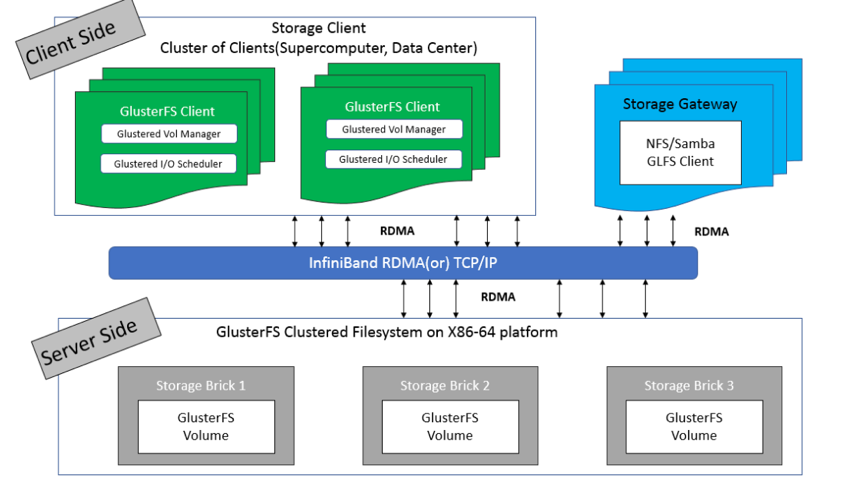
\includegraphics[width=\textwidth]{GlusterFS_Arc}
\caption{GlusterFS整体架构图}
\label{fig:GlusterFS_Arc}
\end{figure}
如图\ref{fig:GlusterFS_Arc}所示,GlusterFS服务端以存储块(Storage Brick)为硬件存储单元,可挂载于磁盘、固态硬盘、内存等多种存储介质。逻辑卷(Volume)是文件系统中的逻辑存储单元,每一个逻辑卷可由一个或者多个存储块构成,绝大多数gluster管理操作是在卷上进行的。GlusterFS根据用户需求能够支持多种逻辑卷,主要包括:

{\color{red}这里itemize的格式有问题}

\begin{itemize}
    \item 分布式卷(Distributed Volume)。文件通过hash算法将数据分布到所有存储服务器上,这种卷是glusterfs的基础和最大特点;其本质功能是扩大的磁盘空间,如果有一个磁盘损坏,其数据也丢失,文件级RAID 0,不具有容错能力。
    \item 复制卷(Replicated Volume)。此类逻辑卷将文件同步复制到多个brick上,文件级RAID 1,具有容错能力,同等硬件条件下写性能下降,但读性能有所提升。
    \item 条带卷(Stripe Volume)。类似RAID0,文件分成数据块以Round Robin方式分布到存储服务器上,并发粒度是数据块,支持超大文件,大文件的读写性能优异。
    \item 复合卷。所谓复合卷主要包括分布式条带卷、分布式复制卷、条带复制卷和分布式条带复制卷等,兼具了基本卷的优点,在实际应用场景下较常见。
\end{itemize}
\begin{figure}[htp]
\centering
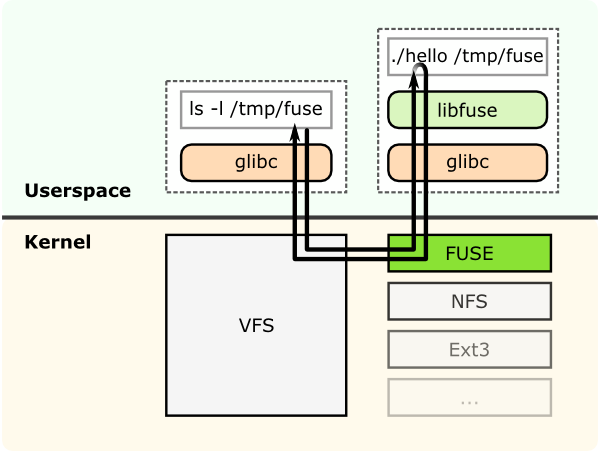
\includegraphics[width=\textwidth]{fuse}
\caption{用户空间文件系统FUSE}
\label{fig:fuse}
\end{figure}
GlusterFS是一个用户空间文件系统,采用了FUSE(File System in Userspace){\color{red}(此处应有引用)}作为用户态程序与内核文件系统交互的接口。如图\ref{fig:fuse}所示,

\subsection{层叠化模块设计Translators}
\begin{figure}[htp]
\centering
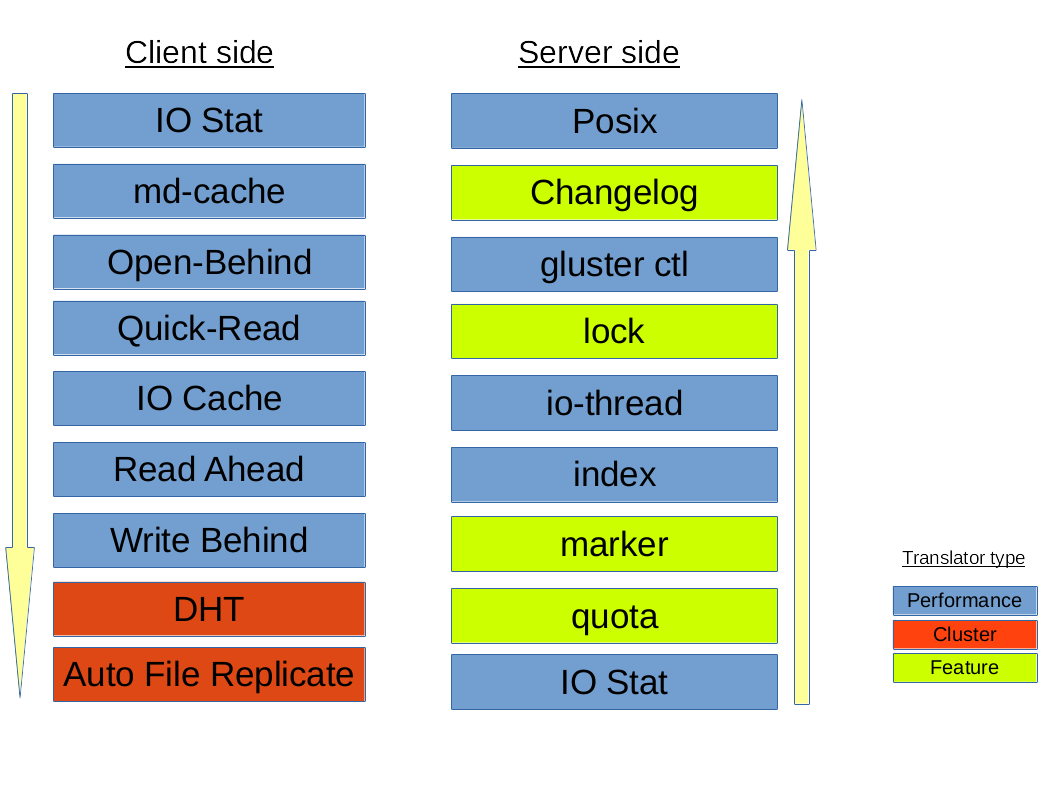
\includegraphics[width=\textwidth]{translators}
\caption{由模块(Translators)堆叠组成的堆栈式结构}
\label{fig:translators}
\end{figure}
Translator是GlusterFS中处理文件请求,实现各类文件操作功能的模块
\cite{BWFS}\cite{DPFS}。
如图\ref{fig:translators}所示,不同功能的模块以动态链接库的方式加载,以函数调用的形式逐级传递和处理文件操作请求,并通过回调函数传回文件操作结果或读取的数据。客户端和服务端之间的消息传递则通过远程过程调用(Remote Procedure Call)实现。
Translator模块是GlusterFS实现诸多功能的主要组件,每一层translator模块内均可对POSIX文件操作函数(打开文件、读写数据和元数据访问等)重新定义,可通过修改参数或修改回调数据等方式实现特定功能。Translator模块以一对一或一对多的方式堆叠组合实现更复杂的功能。

%GlusterFS主要包括cluster,performance,features,protocal,storage,encryption等几类模块。其中cluster类模块是实现存储集群功能的核心,包括分布式哈希表(DHT),
GlusterFS主要包括以下几组translator模块:
\begin{enumerate}
    \item 集群模块组(Cluster Translators)。主要包括分布式哈希表(DHT)、自动文件备份(AFR)等模块,是构成存储服务器集群功能的核心组件。GlusterFS没有采用元数据服务器定位文件数据,而是采用弹性哈希算法定位文件,首先根据文件路径计算哈希值,然后根据哈希值定位到具体的brick存储单元进行文件定位。AFR模块的功能则是自动冗余备份(为避免分歧,通常备份数据多于两个),当发生数据丢失或损坏时进行数据修复。
    \item 性能模块组(Performance Translators)。此类模块的目的是对GlusterFS的整体性能进行优化,如io-cache在GlusterFS进程的内存池内空闲部分开辟空间用于缓存;io-threads用于多线程管理;md-cache用于元数据缓存服务;read-ahead用于预读数据;write-back实现写回功能提升写数据性能等等。
    \item 功能模块组(Feature Translators)。主要包括日志管理模块changelog,全局锁管理locks模块等等。
    \item 协议模块组(Protocol Translators)。GlusterFS架构下,客户端与存储服务端互联方式多种多样,通过协议模块组实现对多种标准协议的支持。
    \item 存储模块组(Storage Translators)。实现GlusterFS与本地POSIX文件系统的接口。
    \item 加密模块组(Encryption Translators)。顾名思义,可以在此类模块中灵活定义不同的加密算法以保证数据安全性。
    \item 调试模块组(Debug Translators)。
\end{enumerate}

\subsection{Tiering模块工作原理}
\begin{figure}[htp]
\centering
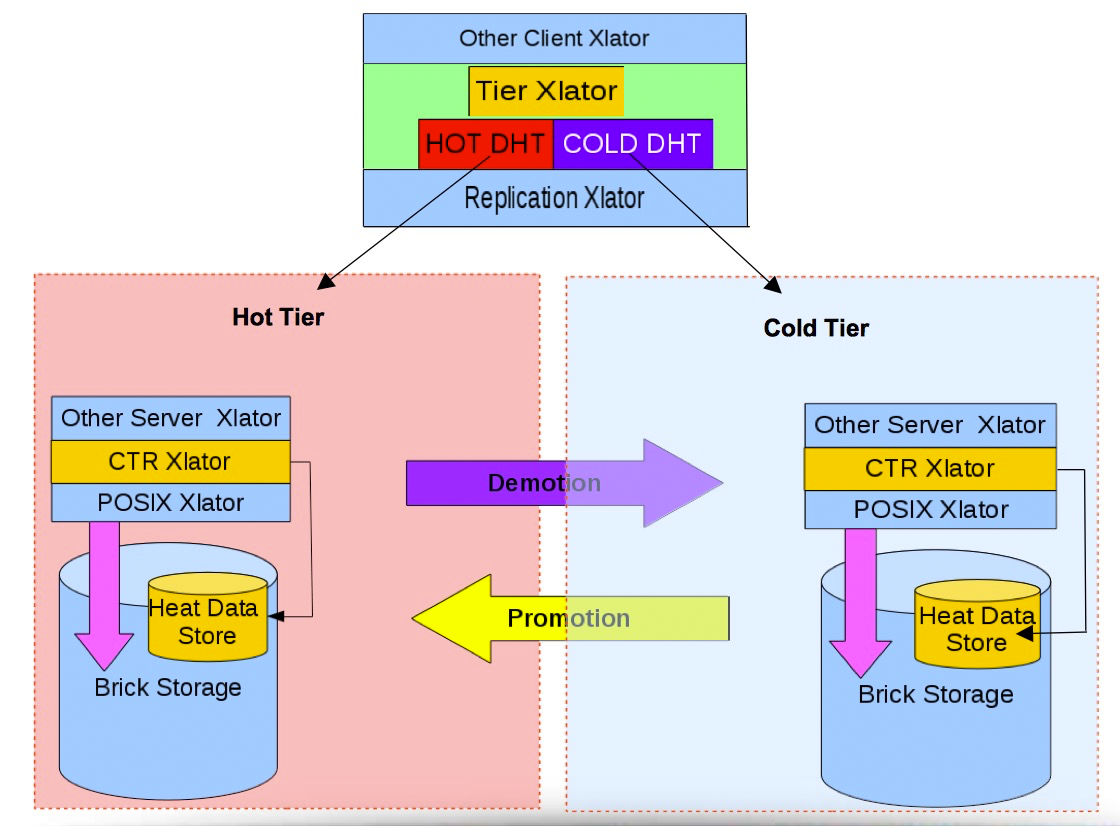
\includegraphics[width=\textwidth]{tiering}
\caption{Tiering模块原理}
\label{fig:tiering}
\end{figure}
Tiering模块是GlusterFS自3.7之后开始支持的分层数据管理模块\cite{Tiering}。与传统分层存储思想类似,文件数据被冠以“热”与“冷”的分类标签,即,访问频繁的文件为“热”数据,反之为“冷”数据。在Tiering模块的实现中,同一逻辑卷被同时挂载到“冷热”两类brick存储单元,“热”存储单元(通常为高性能存储介质如DRAM或SSD等)被视为“冷”存储(廉价、性能较弱的磁盘)的上一级缓存,因此文件的“冷热”对用户应用透明,完全由tiring模块负责文件分类与缓存调度。

如图\ref{fig:tiering},当GlusterFS启用tiering模块时,原本的分布式哈希算法模块被调整为“热”哈希模块与“冷”哈希模块。文件定位与查找优先在“热”存储内进行,若查找成功就是一次缓存命中;反之发生缓存缺失时通过“冷”哈希模块将请求转发到“冷”存储进行重新定位查找。

传统缓存替换算法LRU的实现过程中的核心指标是数据近期访问次数(通常存储于访问速度最快的L1-cache中),近期最少访问的数据被淘汰,而tiering模块则沿用了这一思想。区别在于tiering模块中缓存置换的粒度远远大于CPU cache或内存级的缓存,大多数应用场景是将SSD作为磁盘阵列的缓存,需要迁移置换的数据量大(大文件或海量小文件),同时算法的时间粒度也要宽松得多。

基于上述原因,GlusterFS基于sqlite3实现了一个专门用于记录文件访问记录的数据库libgfdb。该数据库用于记录存储单元内所有已知文件的元数据,作为文件“冷热”分类的依据。

\begin{table}[htbp]
\centering
\begin{minipage}[t]{0.9\linewidth}
\caption{Libgfdb中的元数据结构}
\label{tab:libgfdb_file}
\begin{tabularx}{\linewidth}{cZ}
\toprule[1.5pt]
{\hei 元数据} & 描述\\
\midrule[1pt]
GF\_ID & 文件的GFID\\
W\_SEC, W\_MSEC & 写操作请求发起(wind)时间,以秒或毫秒为单位\\
UW\_SEC, UW\_MSEC & 写操作{\color{red}返回}时间\\
U\_READ\_SEC, W\_READ\_MSEC & 读操作请求发起时间\\
UW\_READ\_SEC, W\_READ\_MSEC & 读操作{\color{red}返回}时间\\
WRITE\_FREQ\_CNTR & 写操作频率\\
READ\_FREQ\_CNTR & 读操作频率\\
\bottomrule[1.5pt]
\end{tabularx}
\end{minipage}
\end{table}

\begin{table}[htbp]
\centering
\begin{minipage}[t]{0.9\linewidth}
\caption{Libgfdb目录入口表(Directory Entries)}
\label{tab:libgfdb_flink}
\begin{tabularx}{\linewidth}{cZ}
\toprule[1.5pt]
元数据 & 描述\\
\midrule[1pt]
GF\_ID & 文件的GFID(复合主键)\\
GF\_PID & 父目录的GFID(复合主键)\\
FNAME & 文件名(复合主键)\\
FPATH & 完整路径\\
W\_DEL\_FLAG & 文件删除(unlinked)标志\\
LINK\_UPDATE & 文件重命名标志\\
\bottomrule[1.5pt]
\end{tabularx}
\end{minipage}
\end{table}

表\ref{tab:libgfdb_file}记录了所有已知文件的访问情况,包括文件操作的起始时间,访问频率等。表\ref{tab:libgfdb_flink}本质上是libgfdb维护的目录入口表,主要用于文件查找。

除“冷热”哈希模块外,另一个关键模块是访问计数器模块CTR(Change Time Recorder)。该模块位于底层POSIX模块之上,其主要功能是对存储单元内所有文件的访问情况进行记录,包括近期内数据读、数据写和元数据写等操作的执行次数等,用于更新libgfdb数据库。

当一个逻辑卷启用tiering模块时,将会在后台开启数据迁移进程。该进程周期性地查询数据库,以获得最近的文件访问情况,从而完成{\color{orange}迁入}(promotion)与{\color{orange}迁出}的数据迁移操作。

在系统运行过程中,数据迁移决策同样受到”热“存储占用率的影响。默认设置下,当“热”存储占用未达到75\%时,即便没有达到周期性迁移的时间节点,系统也会自动将“冷”存储单元内的高频率访问文件迁入“热”存储单元,以防止迁出过多数据导致缓存空间的浪费;当“热”存储占用超过默认的90\%时,将自动地触发迁出操作,以防止到达缓存容量上限降低整体性能。

如上所述,GlusterFS实现的tiering模块主要采用传统的LRU算法设计,能够显著改善大文件的连续读操作,但对于一些不具备“缓存友好”性质的工作负载,例如多客户端并发访问大量小文件的场景下,tiering的性能提升不够明显
\cite{Red_Hat_Gluster_storage_on_supermicro_storage_servers_powered_by_Intel_Xeon_processors}。
其本质原因是随着小文件数量大幅增加,且多客户端的并发文件请求数量上升时,传统缓存置换算法考虑的时间局部性和空间局部性失去效用,仅仅简单地以文件访问频率作为考量不足以分析提取复杂场景下的I/O访问模式。


\section{热点数据识别与数据迁移框架}
%整体框图
\subsection{元数据构造}
\subsection{文件操作追踪}
\subsection{模型训练}
\subsection{运行时数据迁移管理}

\section{本章小结}

% 引言:总框图,描述
% 4.1 客户端设计
% 4.2 服务端设计

\chapter{实验设计与结果分析}
Results
\section{实验环境与工作负载}

\section{实验数据采集与预处理}
\section{实验结果与分析}
\subsection{文件与目录名向量化}
\subsection{门控循环神经网络模型训练与仿真测试}
\section{本章小结}
%gluster tiering 模块实验
%针对工作负载的文件向量化实验(可视化)
%采用循环神经网络进行文件冷热分类
\chapter{总结}
\section{本文工作总结}
\section{未来工作展望}



%%% Local Variables:
%%% mode: latex
%%% TeX-master: "../main"
%%% End:

\begin{ack}
时光荏苒,我的硕士生涯已接进尾声。这几年的时光既漫长又短暂,其中充满了酸甜苦辣,更有收获和成长。几年来,感谢陪我一起度过美好时光的每位尊敬的老师和亲爱的同学,正是你们的帮助,我才能克服困难,正是你们的指导,我才能解决疑惑,直到学业的顺利完成。

本人的学位论文是在我的两位恩师周恩强教授和刘杰教授的殷切关怀和耐心指导下进行并完成的,衷心感谢他们对我的淳淳教诲和悉心关怀。从课题的选择、项目的实施,直至论文的最终完成,恩师始终给予我耐心的指导和支持,我取得的每一点成绩都凝聚着恩师的汗水和心血。恩师开阔的视野、严谨的治学态度、精益求精的工作作风,深深地感染和激励着我,在此谨向他们致以衷心的感谢和崇高的敬意。
  
感谢实验室的师弟师妹们与我一道分享他们青春的快乐!在此还要对实验室所有师兄弟姐妹们在平时开展相关工作中的支持和帮助一并表示感谢。无论在炎热的夏天,还是寒冷的冬季,他们不辞劳苦地为我提供无私的帮助,没有他们的帮助就没有这篇论文的顺利完成。
  
感谢国防科技大学给我提供的平台和机会。今后我会更加努力钻研学术,也更加清醒地意识到必须做终生学习型的人。感谢我的家人常年对我的支持和理解!他们是最爱我的人,也是我亏欠最多的人,他们默默的奉献是我多年来的支持和动力。
  
最后,我要向百忙之中参与审阅、评议本论文各位老师、向参与本人论文答辩的各位老师表示由衷的感谢!人生的每个阶段都值得好好珍惜,这段美好岁月,因为有你们的关心和帮助,我很幸福。我会更加勤奋学习、认真研究,我会努力做得更好,我想这也是我能给你们的最好的回报吧。把最美好的祝福献给你们,愿永远健康、快乐!
\end{ack}


\cleardoublepage
\phantomsection
\addcontentsline{toc}{chapter}{参考文献}
\bibliographystyle{bstutf8}
\bibliography{ref/thesis}

\begin{resume}
%该论文作者在学期间取得的阶段性成果(学术论文等)已满足我校硕士学位评阅相关要求。为避免阶段性成果信息对专家评价学位论文本身造成干扰,特将论文作者的阶段性成果信息隐去。
  \section*{发表的学术论文} % 发表的和录用的合在一起

  \begin{enumerate}[label={[\arabic*]},itemsep=0pt,parsep=0pt,labelindent=26pt,labelwidth=*,leftmargin=0pt,itemindent=*,align=left]
   %[label=\textbf{[\arabic*]},itemindent=*, align=left] %老版本缩进对齐
   
  %\addtolength{\itemsep}{-.36\baselineskip}%缩小条目之间的间距,下面类似
  \item Hui Chen, Enqiang Zhou, Jie Liu, Zhicheng Zhang, et al. An RNN Based Mechanism for File Prefetching. 18th Distributed Computing and Applications for Business Engineering and Science.

  \end{enumerate}
\end{resume}

% 最后,需要的话还要生成附录,全文随之结束。
%\appendix
\backmatter
%% TeX
\chapter{模板提供的希腊字母命令列表}

大写希腊字母:
\begin{table}[htbp]
\centering
\begin{tabular}{llll}
\toprule
$\Gamma$~\verb|\Gamma| & $\Lambda$~\verb|\Lambda| & $\Sigma$~\verb|\Sigma| & $\Psi$~\verb|\Psi| \\
$\Delta$~\verb|\Delta| & $\Xi$~\verb|\Xi| & $\Upsilon$~\verb|\Upsilon| & $\Omega$~\verb|\Omega| \\
$\Theta$~\verb|\Theta| & $\Pi$~\verb|\Pi| & $\Phi$~\verb|\Phi| & \\
\midrule
$\varGamma$~\verb|\varGamma| & $\varLambda$~\verb|\varLambda| & $\varSigma$~\verb|\varSigma| & $\varPsi$~\verb|\varPsi| \\
$\varDelta$~\verb|\varDelta| & $\varXi$~\verb|\varXi| & $\varUpsilon$~\verb|\varUpsilon| & $\varOmega$~\verb|\varOmega| \\
$\varTheta$~\verb|\varTheta| & $\varPi$~\verb|\varPi| & $\varPhi$~\verb|\varPhi| & \\
\bottomrule
\end{tabular}
\end{table}

小写希腊字母:
\begin{table}[htbp]
\centering
\begin{tabular}{llll}
\toprule
$\alpha$~\verb|\alpha| & $\theta$~\verb|\theta| & $o$~\verb|o| & $\tau$~\verb|\tau| \\ 
$\beta$~\verb|\beta| & $\vartheta$~\verb|\vartheta| & $\pi$~\verb|\pi| & $\upsilon$~\verb|\upsilon| \\ 
$\gamma$~\verb|\gamma| & $\iota$~\verb|\iota| & $\varpi$~\verb|\varpi| & $\phi$~\verb|\phi| \\ 
$\delta$~\verb|\delta| & $\kappa$~\verb|\kappa| & $\rho$~\verb|\rho| & $\varphi$~\verb|\varphi| \\ 
$\epsilon$~\verb|\epsilon| & $\lambda$~\verb|\lambda| & $\varrho$~\verb|\varrho| & $\chi$~\verb|\chi| \\ 
$\varepsilon$~\verb|\varepsilon| & $\mu$~\verb|\mu| & $\sigma$~\verb|\sigma| & $\psi$~\verb|\psi| \\ 
$\zeta$~\verb|\zeta| & $\nu$~\verb|\nu| & $\varsigma$~\verb|\varsigma| & $\omega$~\verb|\omega| \\ 
$\eta$~\verb|\eta| & $\xi$~\verb|\xi| & $\varkappa$~\verb|\varkappa| & $\digamma$~\verb|\digamma| \\ 
\midrule
$\upalpha$~\verb|\upalpha| & $\uptheta$~\verb|\uptheta| & $\mathrm{o}$~\verb|\mathrm{o}| & $\uptau$~\verb|\uptau| \\ 
$\upbeta$~\verb|\upbeta| & $\upvartheta$~\verb|\upvartheta| & $\uppi$~\verb|\uppi| & $\upupsilon$~\verb|\upupsilon| \\ 
$\upgamma$~\verb|\upgamma| & $\upiota$~\verb|\upiota| & $\upvarpi$~\verb|\upvarpi| & $\upphi$~\verb|\upphi| \\ 
$\updelta$~\verb|\updelta| & $\upkappa$~\verb|\upkappa| & $\uprho$~\verb|\uprho| & $\upvarphi$~\verb|\upvarphi| \\ 
$\upepsilon$~\verb|\upepsilon| & $\uplambda$~\verb|\uplambda| & $\upvarrho$~\verb|\upvarrho| & $\upchi$~\verb|\upchi| \\ 
$\upvarepsilon$~\verb|\upvarepsilon| & $\upmu$~\verb|\upmu| & $\upsigma$~\verb|\upsigma| & $\uppsi$~\verb|\uppsi| \\ 
$\upzeta$~\verb|\upzeta| & $\upnu$~\verb|\upnu| & $\upvarsigma$~\verb|\upvarsigma| & $\upomega$~\verb|\upomega| \\ 
$\upeta$~\verb|\upeta| & $\upxi$~\verb|\upxi| & & \\ 
\bottomrule
\end{tabular}
\end{table}

希腊字母属于数学符号类别,请用\verb|\bm|命令加粗,其余向量、矩阵可用\verb|\mathbf|。


\end{document}

